\chapter{Disjoint paths with SR}
\label{chapter:disjoint}

\section*{Introduction}

For an Internet Service Provider (ISP), providing disjoint paths to its
customers might be one of those advanced connectivity services that generate
more revenues. This is what emerged from our discussion with a national ISP that
we call ``reference ISP''. When we met them, this ISP's operators themselves
steered the discussion towards possibilities to provide disjoint paths between
sites to which a customer is connected. They were motivated by requests from
banks and financial customers.

We have quickly realized that the disjoint-path connectivity service has a much
bigger market than our reference ISP. An illustration is provided by the
NANOG email discussion about a major outage of the Bell network on August
4th, 2017~\cite{refnanog}. The email thread started with Bell's customers
complaining that both Internet and mobile connectivity were completely absent in
East Canada, affecting banking, ATM, land lines and even 911 services. When a
single fibre cut was indicated as the cause of the outage, someone expressed
doubts that ISPs really provide geographically diverse circuits, irrespectively
of what they promise and sell. The following emails discussed the impossibility
to work around this limitation by relying on two providers, as their networks
may share the same physical infrastructure (fibres, conduit, etc.), without the
ISPs even knowing it -- as they do not share information between each other.

The discussion we had with the reference ISP's operators was indeed focused on
\textit{providing disjoint paths within a single ISP}, their own. A possible
solution~\cite{art:2014} to achieve this goal is to deploy two parallel
networks, say a red and a blue copy of the same topology, and configure the
intra-domain routing protocol (IGP) so that any packet is forwarded in only one of
the two networks -- i.e., packets that enter the red copy are only forwarded in
the red copy.
The few links between the two networks are only used if one of the two copies is
partitioned. This architecture provides disjoint paths by design, but it is very
expensive since the entire network is doubled.
The reference ISP's operators were therefore reluctant to deploy it.
%The operators discarded solutions
%based on adding physical redundancy, like the 1+1 protection scheme in optical
%networks~\cite{}, because of the additional costs. 
Of course, they were also aware that MPLS tunnels can be created over
arbitrary paths with RSVP-TE~\cite{rfc3209}, including disjoint ones, on an
existing infrastructure.
However, they were in the process of moving away from MPLS, in order to avoid
its operational limitations~\cite{mpls-opissues-ripe64}, its sub-optimal usage
of resources~\cite{mpls-latency-imc11} and its scalability challenges with
respect to the routers' state~\cite{rfc5439,defo-sig15}.

%including synchronization with the
%underlying IGP and control-plane overhead~\cite{}, scalability~\cite{} and
%latency inflation~\cite{mpls-latency-imc11}.

Looking at other ISPs, our operators were instead considering Segment Routing
(SR). Motivated by this, we dedicate this chapter to the study of the problem of computing and implementing disjoint paths over a network
with segment routing. We also provide a solution for leveraging some properties of sr-paths to
show how we can provide disjoint paths that are robust to link failures.


\section{Disjoint paths and network flows}
\label{section:dp}

The problem of computing disjoint paths in a graph is one of those ubiquitous problem that has driven
a lot of research over the years. Numerous algorithms exist for solving it, most of them being some variant
of the more general maximum flow problem \cite{suurballe1984quick, Ahuja}.

The maximum flow problem is the problem of finding the maximum amount of information that can
be sent between two given nodes in a network. It is closely related to the multi-commodity flow
problem that we studied in Chapter \ref{chapter:te}. Instead of being given a set of demands, we are given
a source $s \in V(G)$ and a destination $t \in V(G)$ and we are asked what is the maximum amount of traffic that can be routed 
between those two nodes without exceeding the capacity of any edge. Another way to see it is to 
imagine that we have an infinite amount of unit demands between $s$ and $t$ and we are asked what is the maximum
number of such demands that can simultaneously be routed of the network without exceeding any link capacity.

The maximum flow problem admits an IP formulation that is very similar to the formulation that we gave for the MCF. If we let $x_e$
define the amount of demands routed over edge $e$ it can be shown that the following LP models the problem \cite{Ahuja}.

\begin{center}
\begin{tabular}{crcllr}
\multicolumn{5}{l}{$\maxflow(G, s, t)$} \\[0.5cm] 
$\displaystyle \mathbf{max}$ & $\displaystyle \sum_{e \in \oute(s)} x_e$ & & & & \\[0.5cm]
$\textbf{s.t.}$ & $\displaystyle \sum_{e \in \delta^-(v)} x_{e} - \sum_{e \in \delta^+(v)} x_{e}$ & $=$    & $ 0$ & $\forall v \in V(G) \setminus \{ s, t \}$  &  \\[0.5cm]
                & $x_{e}$ & $\leq$ & $\bnd(e)$ & $\forall e \in E(G)$ & \\[0.5cm]
                & $x_{e}$ & $\in$ & $\mathbb{N}$
\end{tabular}
\end{center}

It is possible to show that the linear programming relaxation of this problem obtained by replacing $x_e \in \mathbb{N}$ by $x_e \geq 0$ 
is equivalent as long as the capacities are integral \cite{Ahuja}. This makes the maximum flow problem one of those rare cases where the integrality constraints no not increase the difficulty
of the problem. Numerous polynomial time algorithms have been developed for solving the maximum flow problem \cite{Edmonds:1972:TIA:321694.321699, dinitz, Goldberg:1988:NAM:48014.61051, Ahuja}.
If we set \emph{unit capacities} on the edges and think about the maximum flow problem as one answering the question of what is the maximum amount of unit demands that we can
route from $s$ to $t$, we see that we actually end up with the \emph{maximum number of disjoint path between $s$ and $t$}. This is the case
since each of the routed demands must follow a path that shares no edges with any of the other demand paths or otherwise some edge would carry at least two units
of traffic, thus exceeding its capacity.

In other words, this means that we can model the problem of computing the maximum number of edge-disjoint paths between $s$ and $t$ by replacing $\bnd(e)$
by $1$ in the $\maxflow$ model. By doing so, we obtain the following model which can also be solved efficiently.

\begin{center}
\begin{tabular}{crcllr}
\multicolumn{5}{l}{$\maxedp(G, s, t)$} \\[0.5cm] 
$\displaystyle \mathbf{max}$ & $\displaystyle \sum_{e \in \oute(s)} x_e$ & & & & \\[0.5cm]
$\textbf{s.t.}$ & $\displaystyle \sum_{e \in \delta^-(v)} x_{e} - \sum_{e \in \delta^+(v)} x_{e}$ & $=$    & $ 0$ & $\forall v \in V(G) \setminus \{ s, t \}$  &  \\[0.5cm]
                & $x_{e}$ & $\leq$ & $1$ & $\forall e \in E(G)$ & \\[0.5cm]
                & $x_{e}$ & $\in$ & $\mathbb{N}$
\end{tabular}
\end{center}

This model focuses solely one providing a maximum amount of paths. It does not care about the quality of those paths, for instance, in terms of latency. It turns out that if we wish to
minimize total latency of the path set we can still do it in polynomial time. This problem is known, in general, as the minimum cost maximum flow problem \cite{Ahuja}.
We can easily adapt the above model to obtain a set of $n$ disjoint paths (if they exist) whose total latency is as small as possible by
requiring the total flow out of $s$ to be $n$ and minimizing the sum of the latencies of the edges with a non-zero flow as shown in the following model.

\begin{center}
\begin{tabular}{crcllr}
\multicolumn{5}{l}{$\minlatedp(G, s, t)$} \\[0.5cm] 
$\displaystyle \mathbf{min}$ & $\displaystyle \sum_{e \in E(G)} \lat(e) \cdot x_e$ & & & & \\[0.5cm]
$\textbf{s.t.}$ & $\displaystyle \sum_{e \in \delta^-(v)} x_{e} - \sum_{e \in \delta^+(v)} x_{e}$ & $=$    & $ 0$ & $\forall v \in V(G) \setminus \{ s, t \}$  &  \\[0.5cm]
                & $\displaystyle \sum_{e \in \oute(s)} x_e$ & $=$ & $n$ & \\[0.5cm]
                & $x_{e}$ & $\leq$ & $1$ & $\forall e \in E(G)$ & \\[0.5cm]
                & $x_{e}$ & $\in$ & $\mathbb{N}$
\end{tabular}
\end{center}

If we want $n$ to be as large as possible we can simply first compute the optimal solution of $\maxedp(G, s, t)$ and set $n$ to that value.
Surprisingly, this problem can also be solved in polynomial time \cite{Ahuja}. Unfortunately, slight variations of this problem that are of interest for computer
networks quickly become \NPhard. For instance, if we want to minimize the maximum latency over all the paths rather than the latency sum, the problem is 
\NPhard~even if $n = 2$ \cite{minmax-disjoint-90, Li1990}. Another change that, perhaps surprisingly, makes the problem \NPhard~is to have two origins $s_1, s_2$ and two destinations
$t_1, t_2$ and ask for a pair of disjoint paths, one from $s_1$ to $t_1$ and another from $s_2$ to $t_2$ \cite{VYGEN199583}. One might naively think that we could get away by adding a fake node 
$s$ linked to both $s_1, s_2$ and link $t_1, t_2$ to some other fake $t$ and then compute the maximum flow from $s$ to $t$. Unfortunately, nothing in the model
forces the flow originating from $s_1$ to go to $t_1$ instead of $t_2$ (and vice-versa). In order to force some origin to destination assignment, we cannot rely on a
maximum flow model but rather on a multi-commodity flow model which, as we have already seen, is harder to solve. 


\section{Disjoint sr-paths}
\label{section:dpsr}

In the previous section we talked about the general problem of finding sets of disjoint paths over a network.
However, the paths found by these algorithms can be arbitrary and thus hard to implement with segment 
routing as we will show shortly.

In this section we redefine the problem in terms of segment routing and adapt the MIP models from
the previous section accordingly. We start by defining what disjoint sr-path are and the problem of finding
a maximum cardinality set of sr-paths.

\begin{definition}
Let $G$ be a network and $\sr{p}, \sr{q}$ be two sr-paths on $G$. We say that $\sr{p}$ and $\sr{q}$ are \emph{disjoint} if
$E(\sr{p}) \cap E(\sr{q}) = \emptyset$. 
\end{definition}

\begin{problem}{Maximum edge-disjoint sr-paths problem}
\label{prob:max-sr-edp}
\textbf{Input:} A network $G$, two nodes $s, t \in V(G)$ and $k \in \mathbb{N}$.

\textbf{Output:} A set of sr-paths $\{ \sr{p}_1, \ldots, \sr{p}_n \} \subseteq \Pk(s, t)$ such that for each $i \neq j$, $\sr{p}_i$ and $\sr{p}_j$
are disjoint and $n$ is maximum.
\end{problem}

Recall that in case of ECMP between two consecutive segments of $\sr{p}$, the set $E(\sr{p})$ contains the edges belonging to \emph{all} 
those ECMP paths. In other words, we are requiring all those shortest paths corresponding to $\sr{p}$ and $\sr{q}$ to be edge-disjoint.
This is necessary because we can never be sure where exactly the traffic will flow when using a sr-path. In this way, we ensure that no matter how traffic is routed
over ECMPs, no edge will carry packets from two distinct sr-paths $\sr{p}_i$ and $\sr{p}_j$. Figure \ref{fig:non-disjoint} illustrates this with source node $\node{a}$
and destination node $\node{h}$. The two sr-paths displayed
on it are not disjoint because there might both use edge $(\node{e}, \node{h})$ in the event of the green one using path 
$(\edge{a}{c}, \edge{c}{d}, \edge{d}{e}, \edge{e}{h})$ and the blue one using $(\edge{a}{b}, \edge{b}{e}, \edge{e}{h})$.
This can be prevented by, for instance, forcing the blue path to pass thought node $\node{f}$ as shown in Figure \ref{fig:disjoint}.

\begin{figure}
\begin{center}
\begin{tikzpicture}
\def\x{0}
\def\y{0}

\node[scale=0.15] (a) at (0.5 + \x,  0.5 + \y) {\router{a}{router}};
\node[scale=0.15] (b) at (0.5 + \x, -1.0 + \y) {\router{b}{router}};
\node[scale=0.15] (c) at (2.5 + \x,  0.0 + \y) {\router{c}{router}};
\node[scale=0.15] (d) at (4.5 + \x,  0.0 + \y) {\router{d}{router}};
\node[scale=0.15] (e) at (4.0 + \x, -2.0 + \y) {\router{e}{router}};
\node[scale=0.15] (g) at (6.0 + \x,  0.5 + \y) {\router{g}{router}};
\node[scale=0.15] (i) at (8.0 + \x,  0.0 + \y) {\router{i}{router}};
\node[scale=0.15] (h) at (7.0 + \x, -1.5 + \y) {\router{h}{router}};
\node[scale=0.15] (f) at (4.0 + \x, -3.5 + \y) {\router{f}{router}};
\node[scale=0.15] (j) at (8.0 + \x, -2.5 + \y) {\router{j}{router}};
\draw[line width=2] (a) edge[above, sloped] node[black] {} (b);
\draw[line width=2]  (a) edge[above, sloped] node[black] {} (c);

\draw[line width=2] (b) edge[above, sloped] node[black] {} (c);
\draw[line width=2] (b) edge[above, sloped] node[black] {} (e);
\draw[line width=2] (b) edge[above, sloped] node[black] {} (f);
\draw[line width=2]  (c) edge[above, sloped] node[black] {} (d);
\draw[line width=2]  (d) edge[above, sloped] node[black] {} (e);
\draw[line width=2]  (d) edge[above, sloped] node[black] {} (g);
\draw[line width=2] (e) edge[above, sloped] node[black] {} (c);
\draw[line width=2] (e) edge[above, sloped] node[black] {} (f);
\draw[line width=2] (f) edge[above, sloped] node[black] {} (j);
\draw[line width=2] (f) edge[above, sloped] node[black] {} (h);
\draw[line width=2] (g) edge[above, sloped] node[black] {} (i);
\draw[line width=2]  (g) edge[above, sloped] node[black] {} (h);
\draw[line width=2] (h) edge[above, sloped] node[black] {} (j);
\draw[line width=2] (i) edge[above, sloped] node[black] {} (h);
\draw[line width=2, red]  (e) edge[above, sloped] node[black] {} (h);

\draw[line width=3, darkgreen]  (a) edge[above, bend left=15, sloped, ->] node[black] {} (c);
\draw[line width=3, darkgreen]  (c) edge[above, bend left=15, sloped, ->] node[black] {} (d);
\draw[line width=3, darkgreen]  (d) edge[above, bend left=15, sloped, ->] node[black] {} (g);
\draw[line width=3, darkgreen]  (d) edge[above, bend right=15, sloped, ->] node[black] {} (e);
\draw[line width=3, darkgreen]  (e) edge[above, bend left=15, sloped, ->] node[black] {} (h);
\draw[line width=3, darkgreen]  (g) edge[above, bend left=15, sloped, ->] node[black] {} (h);

\draw[line width=3, cyan]  (a) edge[above, bend right=15, sloped, ->] node[black] {} (b);
\draw[line width=3, cyan]  (b) edge[above, bend right=15, sloped, ->] node[black] {} (e);
\draw[line width=3, cyan]  (b) edge[above, bend right=15, sloped, ->] node[black] {} (f);
\draw[line width=3, cyan]  (f) edge[above, bend right=15, sloped, ->] node[black] {} (h);
\draw[line width=3, cyan]  (e) edge[above, bend right=15, sloped, ->] node[black] {} (h);

\node[draw, fill=cyan!20!white, left = 0.1cm of a] (x1) {\small $x_1$};
\node[draw, fill=cyan!20!white, left = 0.1cm of b] (x2) {\small $x_2$};
\node[draw, fill=cyan!20!white, right = 0.1cm of h] (x3) {\small $x_3$};

\node[draw, fill=green!50!white, above = 0.1cm of a] (y1) {\small $y_1$};
\node[draw, fill=green!50!white, above = 0.1cm of d] (y2) {\small $y_2$};
\node[draw, fill=green!50!white, above = 0.1cm of x3] (y3) {\small $y_3$};


\end{tikzpicture}
\end{center}
\caption{The sr-paths $\langle \node{a}, \node{d}, \node{h} \rangle$ and $\langle \node{a}, \node{b}, \node{h} \rangle$ are not edge-disjoint
because their edge sets intersect over $(\node{e}, \node{h})$.}
\label{fig:non-disjoint}
\end{figure}


\begin{figure}
\begin{center}
\begin{tikzpicture}
\def\x{0}
\def\y{0}

\node[scale=0.15] (a) at (0.5 + \x,  0.5 + \y) {\router{a}{router}};
\node[scale=0.15] (b) at (0.5 + \x, -1.0 + \y) {\router{b}{router}};
\node[scale=0.15] (c) at (2.5 + \x,  0.0 + \y) {\router{c}{router}};
\node[scale=0.15] (d) at (4.5 + \x,  0.0 + \y) {\router{d}{router}};
\node[scale=0.15] (e) at (4.0 + \x, -2.0 + \y) {\router{e}{router}};
\node[scale=0.15] (g) at (6.0 + \x,  0.5 + \y) {\router{g}{router}};
\node[scale=0.15] (i) at (8.0 + \x,  0.0 + \y) {\router{i}{router}};
\node[scale=0.15] (h) at (7.0 + \x, -1.5 + \y) {\router{h}{router}};
\node[scale=0.15] (f) at (4.0 + \x, -3.5 + \y) {\router{f}{router}};
\node[scale=0.15] (j) at (8.0 + \x, -2.5 + \y) {\router{j}{router}};
\draw[line width=2] (a) edge[above, sloped] node[black] {} (b);
\draw[line width=2]  (a) edge[above, sloped] node[black] {} (c);

\draw[line width=2] (b) edge[above, sloped] node[black] {} (c);
\draw[line width=2] (b) edge[above, sloped] node[black] {} (e);
\draw[line width=2] (b) edge[above, sloped] node[black] {} (f);
\draw[line width=2]  (c) edge[above, sloped] node[black] {} (d);
\draw[line width=2]  (d) edge[above, sloped] node[black] {} (e);
\draw[line width=2]  (d) edge[above, sloped] node[black] {} (g);
\draw[line width=2] (e) edge[above, sloped] node[black] {} (c);
\draw[line width=2] (e) edge[above, sloped] node[black] {} (f);
\draw[line width=2] (f) edge[above, sloped] node[black] {} (j);
\draw[line width=2] (f) edge[above, sloped] node[black] {} (h);
\draw[line width=2] (g) edge[above, sloped] node[black] {} (i);
\draw[line width=2]  (g) edge[above, sloped] node[black] {} (h);
\draw[line width=2] (h) edge[above, sloped] node[black] {} (j);
\draw[line width=2] (i) edge[above, sloped] node[black] {} (h);
\draw[line width=2]  (e) edge[above, sloped] node[black] {} (h);

\draw[line width=3, darkgreen]  (a) edge[above, bend left=15, sloped, ->] node[black] {} (c);
\draw[line width=3, darkgreen]  (c) edge[above, bend left=15, sloped, ->] node[black] {} (d);
\draw[line width=3, darkgreen]  (d) edge[above, bend left=15, sloped, ->] node[black] {} (g);
\draw[line width=3, darkgreen]  (d) edge[above, bend right=15, sloped, ->] node[black] {} (e);
\draw[line width=3, darkgreen]  (e) edge[above, bend left=15, sloped, ->] node[black] {} (h);
\draw[line width=3, darkgreen]  (g) edge[above, bend left=15, sloped, ->] node[black] {} (h);

\draw[line width=3, cyan]  (a) edge[above, bend right=15, sloped, ->] node[black] {} (b);
\draw[line width=3, cyan]  (b) edge[above, bend right=15, sloped, ->] node[black] {} (f);
\draw[line width=3, cyan]  (f) edge[above, bend right=15, sloped, ->] node[black] {} (h);

\node[draw, fill=cyan!20!white, left = 0.1cm of a] (x1) {\small $x_1$};
\node[draw, fill=cyan!20!white, left = 0.1cm of b] (x2) {\small $x_2$};
\node[draw, fill=cyan!20!white, below = 0.1cm of f] (x3) {\small $x_3$};
\node[draw, fill=cyan!20!white, right = 0.1cm of h] (x4) {\small $x_4$};

\node[draw, fill=green!50!white, above = 0.1cm of a] (y1) {\small $y_1$};
\node[draw, fill=green!50!white, above = 0.1cm of d] (y2) {\small $y_2$};
\node[draw, fill=green!50!white, above = 0.1cm of x4] (y3) {\small $y_3$};


\end{tikzpicture}
\end{center}
\caption{The sr-paths $\langle \node{a}, \node{d}, \node{h} \rangle$ and $\langle \node{a}, \node{b}, \node{f}, \node{h} \rangle$ are edge-disjoint.}
\label{fig:disjoint}
\end{figure}

If we ignore the segmentation cost constraints from Problem \ref{prob:max-sr-edp}, the
simplest algorithm to compute a set of edge-disjoint sr-paths is to leverage the minimum segmentation algorithm proposed
in Chapter \ref{chapter:sr} to segment the set of paths produced by the minimum cost flow algorithm. As usual with this
kind of approach, this solution has the drawback of granting no control over the segment cost of the output. For this reason,
we start by analyzing the distribution of the costs over all topologies.
For each topology in our dataset and each pair of distinct nodes, we used a minimum cost maximum flow algorithm to
compute the maximum number of disjoint paths between those nodes whose total latency is as small as possible. Then, we segment each
of those paths and compute the maximum number of segments required to implement those paths on the network. Figure \ref{fig:minCostEDP_segcost}
shows the distribution of the segment costs. We observe that for more than $20\%$ of the pairs we need $6$ or more segments. This motivated
us to propose solutions that are able to limit the number of segments in the output.

\begin{figure}
\begin{center}
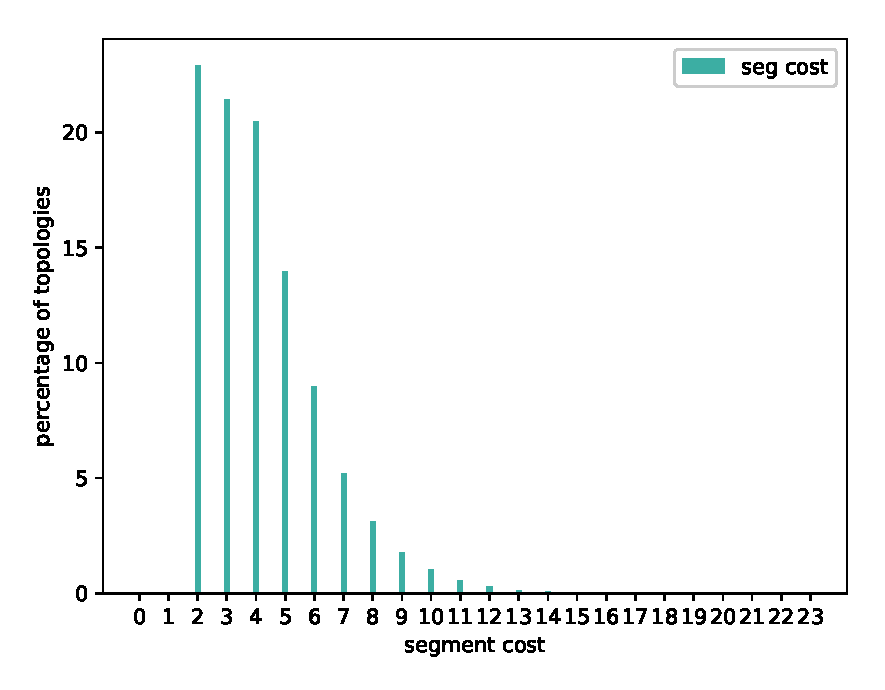
\includegraphics[width=.85\columnwidth]{./Network-lib/data/plot/minCostEDP_segcost.eps}
\end{center}
\caption{Distribution of the maximum segment of maximum cardinality sets of disjoint paths with total minimum latency.}
\label{fig:minCostEDP_segcost}
\end{figure}

\subsection{Maximum set of disjoint sr-paths}

We propose two MIP models for adapting the graph model $\maxedp(G, s, t)$ to Problem \ref{prob:max-sr-edp}. We start by defining
an indicator function telling use whether an edge belongs to the shortest paths between two given nodes.
That is, let $I$ to denote a function $V(G)^2 \times E(G) \rightarrow \{0, 1\}$ defined such that $I(u, v, e) = 1$ if and only if $e \in E(\sp(u, v))$.

Our first model is an adaptation of the traffic engineering segment model $\srteseg(G, \mathcal{D})$ proposed in Chapter \ref{chapter:te}. 
Our demand set contains unit demands between $s$ and $t$. Each such demand corresponds to a sr-path that is edge-disjoint from the
others. We can select the number of demands to be equal to the out-degree of $s$, since this is an upper bound on the number
of disjoint paths from $s$ to any other node. Our objective will by to route a maximum
amount of demands in a way such that no two demands are routed over the same edge. We use variables $x^d_{uv}$ 
saying whether $\sp(u, v)$ is used by the sr-path corresponding to demand $d$. We replace the capacity constraints
by disjointness constraints which consists of requiring that for each edge, at most one demand is routed over it. The rest of the model
is the same as $\srteseg(G, \mathcal{D})$ which uses flow constraints to ensure that paths go from $s$ to $t$.

\begin{center}
\begin{tabular}{rcllr}
\multicolumn{5}{l}{$\sredpseg(G, s, t)$} \\[0.5cm] 
\multicolumn{3}{l}{$\mathbf{max} \quad \displaystyle \sum_{u \in V(G)} \sum_{d = 1}^r x^d_{su}$} & $\textbf{s.t.}$ & \\[0.5cm]
%\multicolumn{5}{l}{{\color{gray!80!white} qsdqsd qsdqsaz sqd s dazz azeqsd azee aze qsd }} \\
$\displaystyle \sum_{d = 1}^r \sum_{u \in V(G)} \sum_{v \in V(G)}  x^d_{uv} \cdot I(u, v, e)$ & $\leq$ & $1$ & $\forall e \in E(G)$ & \\[0.5cm]
$\displaystyle \sum_{u \in V(G) \setminus \{ v \}} x^d_{uv} - \sum_{u \in V(G) \setminus \{ v \}} x^d_{vu}$ & $=$    &  $0$ & $\forall d$, & \\[-0.2cm]
& & & $\forall v \in V(G) \setminus \{ s, t \}$ & \\[0.5cm]
$\displaystyle \sum_{d = 1}^r \sum_{u \in V(G) } x^d_{us} + x^d_{tu}$ & $=$    &  $0$ & $\forall d \in \{1, \ldots, |\oute(s)|\}$ \\[0.5cm] 
$\displaystyle \sum_{u \in V(G)} \sum_{v \in V(G)} x^d_{uu}$ & $\leq$    &  $k$ & $\forall d \in \{ 1, \ldots, |\oute(s)| \}$, \\[0.5cm]
$x^d_{uv}$  &    $\in$    &  $\{0, 1\}$  & $\forall e \in E(G),$ & \\
  &    &   & $\forall d \in \{1, \ldots, |\oute(s)|\}$ &
\end{tabular}
\end{center}

Next, we propose another model whose original idea is due to
Bernard Fortz. After we will compare both models. Note that both these models only support node segments
in the sr-paths.

%For simplicity, we start by presenting the model for sr-paths consisting
%only on node segments. We will describe later how to extend it to also take into account
%adjacency segments as well. 
%As it was already observed by Renauld Hartert, a sr-path 
%consisting only on node segments can between seen as a path on the complete graph
%with $V(G)$ nodes. The correspondence is quite clear as a sr-path with only node segments
%is a sequence $\langle x_1, \ldots, x_l \rangle$ such that each $x_i \in V(G)$ and a
%path on the complete graph also is a sequence $(v_1, \ldots, v_r)$ with each $v_i \in V(G)$.
A sr-path with only node segments is a sequence $\langle y_1, \ldots, y_l \rangle$
such that each $y_1, \ldots, y_l \in V(G)$. The idea behind Fortz  model is to define binary variables 
$x^i_{uv}$ such that $x^i_{uv} = 1$ if and only if
$u$ and $v$ appear as consecutive segments $y_i = u$ and $y_{i + 1} = v$ of a sr-path used in the solution.
These variables are defined for $i = 1, \ldots, k - 1$ where $k$ is the maximum segment cost that we
want to allow the paths to have. Consider for instance that we have a solution where
$x^1_{sa} = x^2_{ab} = x^3_{bt} = 1$. This will correspond to using the sr-path $\langle s, a, b, t\rangle$
as shown in Figure \ref{fig:modelfortz}. So, basically, the index $i$ is saying the position at which we use
each segment.
Note that a more intuitive model would be to drop the $i$ index and use variables $x_{uv}$ to mean that we use
the shortest paths between $u$ and $v$ to route traffic. By adding flow conservation constraints similar to the
ones used in model $\maxflow(G, s, t)$ we can make sure that these variables actually come together
to constitute sr-paths. However, this gives no way of restricting the segment cost of those paths.


\begin{figure}
\begin{center}
\begin{tikzpicture}
\draw[gray, dashed] (0, 0) -- (0, 5) node[anchor=south] {$i = 1$};
\draw[gray, dashed] (2, 0) -- (2, 5) node[anchor=south] {$i = 2$};
\draw[gray, dashed] (4, 0) -- (4, 5) node[anchor=south] {$i = 3$};
\draw[gray, dashed] (6, 0) -- (6, 5) node[anchor=south] {$i = 4$};
\node[scale=0.15] (s) at (-1, 2.5) {\router{s}{router}};
\node[scale=0.15] (a) at (1, 4) {\router{$a$}{router}};
\node[scale=0.15] (b) at (3, 3.5) {\router{$b$}{router}};
\node[scale=0.15] (t1) at (5, 3.75) {\router{$t$}{router}};

\node[scale=0.15] (c) at (1, 5 - 4 - 0.5) {\router{$c$}{router}};
\node[scale=0.15] (d) at (3, 5 - 3.5 - 0.5) {\router{$d$}{router}};
\node[scale=0.15] (e) at (5, 5 - 3.75 - 0.5) {\router{$e$}{router}};
\node[scale=0.15] (t2) at (7, 2.5) {\router{$t$}{router}};


\draw (s) edge[line width=2, above, sloped, ->] node {\small $x^1_{s a} = 1$} (a);
\draw (a) edge[line width=2, above, sloped, ->] node {\small $x^2_{a b} = 1$} (b);
\draw (b) edge[line width=2, above, sloped, ->] node {\small $x^3_{b t} = 1$} (t1);

\draw (s) edge[line width=2, above, sloped, ->] node {\small $x^1_{s c} = 1$} (c);
\draw (c) edge[line width=2, above, sloped, ->] node {\small $x^2_{c d} = 1$} (d);
\draw (d) edge[line width=2, above, sloped, ->] node {\small $x^3_{d e} = 1$} (e);
\draw (e) edge[line width=2, above, sloped, ->] node {\small $x^4_{e t} = 1$} (t2);

\node[right = 0.1cm of t2] {$\langle s, c, d, e, t \rangle$};
\node[right = 0.1cm of t1] {$\langle s, a, b, t \rangle$};
\end{tikzpicture}
\end{center}
\caption{Two examples of how the variables $x^i_{uv}$ define sr-paths.}
\label{fig:modelfortz}
\end{figure}

\begin{center}
\begin{tabular}{crcllr}
\multicolumn{5}{l}{$\sredpfortz(G, s, t)$} \\[0.5cm] 
$\displaystyle \mathbf{max}$ & $\displaystyle \sum_{u \in V(G)} x^1_{su}$ & & & & \\[0.5cm]
$\textbf{s.t.}$ & $\displaystyle \sum_{i = 1}^k \sum_{u \in V(G)} \sum_{v \in V(G)} I(u, v, e) \cdot x^i_{uv} $ & $\leq$    & $1$ & $\forall e \in E(G)$  & $(1)$ \\[0.5cm]
                & $\displaystyle \sum_{v \in V(G)} x^{i - 1}_{vu} - \sum_{v \in V(G)} x^i_{uv}$ & $=$ & $0$ & $\forall u \in V(G) \setminus \{s, t\}$, &  $(2)$ \\[-0.2cm] 
                & & & & $i = 2, \ldots, k$ &  \\[0.5cm] 
                & $\displaystyle \sum_{i = 1}^k \sum_{v \in V(G)} x^i_{vs} + x^i_{tv}$ & $=$ & $0$ &  & $(3)$ \\[0.5cm]
                & $\displaystyle \sum_{v \in V(G) \setminus \{s\}} x^1_{vu} + \sum_{v \in V(G) \setminus \{t\}} x^k_{uv}$ & $=$ & $0$ & $\forall u \in V(G)$ & $(4)$\\[0.5cm]
                & $x_{e}$ & $\in$ & $\mathbb{N}$
\end{tabular}
\end{center}

Constraints $(1)$ ensure that each edge is used only once making sure that the final paths are indeed edge-disjoint. Recall that setting $x^{i - 1}_{uv}$ to $1$ means that
node $u$ is used as a node segment at position $i - 1$ in some sr-path in the solution. Thus, if $u \neq t$ we need to make sure that there is also some node $v'$ coming after $u$ in this sr-path as
illustrated in Figure \ref{fig:modelfortz2}. This is what constraints $(2)$ ensure, that is, that for each $u$ such that $x^{i - 1}_{vu}$ for some $v$, there is also some element
$v'$ such that $x^{i}_{uv'}$ ensuring that the path does not end at a node $u \neq t$. 
These constraints are similar to the classical conservation constraints that are commonly used in these kinds of models to ensure connectivity.



\begin{figure}
\begin{center}
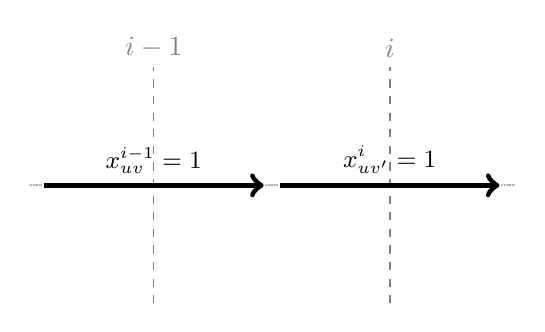
\begin{tikzpicture}
\draw[gray, dashed] (1, 1) -- (1, 4) node[anchor=south] {$i - 1$};
\draw[gray, dashed] (4, 1) -- (4, 4) node[anchor=south] {$i$};
\node[scale=0.15] (v) at (-0.5, 2.5) {\router{$v$}{router}};
\node[scale=0.15] (u) at (2.5, 2.5) {\router{$u$}{router}};
\node[scale=0.15] (v2) at (5.5, 2.5) {\router{$v'$}{router}};

\draw (v) edge[line width=2, above, sloped, ->] node {\small $x^{i - 1}_{uv} = 1$} (u);
\draw (u) edge[line width=2, above, sloped, ->] node {\small $x^{i}_{uv'} = 1$} (v2);

\end{tikzpicture}
\end{center}
\caption{If $x^{i - 1}_{uv} = 1$ .}
\label{fig:modelfortz2}
\end{figure}

Constraints $(3)$ simply make sure that $s$ appears only as the first element of the sr-paths and that $t$ occurs only as the last one.
Finally, constraints $(4)$ prevent other nodes to be the starting and end-points of paths by ensuring that $x^1_{uv}$ can only be set if $u = s$
and that $x^k_{uv}$ can only be set if $v = t$.

Figure \label{fig:maxEDP_runtime} shows a CDF of the runtime needed to compute optimal solutions of $\sredpseg(G, s, t)$  and $\sredpfortz(G, s, t)$ using Gurobi. In
both cases the maximum number of segments was set to $5$. We generated
$100$ random source-destination pairs and solved both models over these pairs for all instances in our dataset. We can see (in orange) that the segment
model is slower than the model proposed by Fortz (in blue). We see that the maximum runtime of the Fortz model is about $3$ minutes whereas
the maximum runtime of the segment model is about $10$ minutes. In both cases this shows that using a MIP solver for computing sets of disjoint
sr-paths is feasible in practice in a reasonable amount of time. 
In order to try to understand whether our sample of $100$ pairs is large enough, we computed a box-plot of the run times on the topologies from groups
\texttt{real} and \texttt{rf} of the Fortz model. 
We selected these because they are the largest ones and we cannot show all results in the box plot. Figure \ref{fig:maxEDP_boxplot} shows these. Except for
topology \texttt{1239}, the runtime does not have a high variance so we can expect that the average runtime is close
to the one computed.

\begin{figure}
\begin{center}
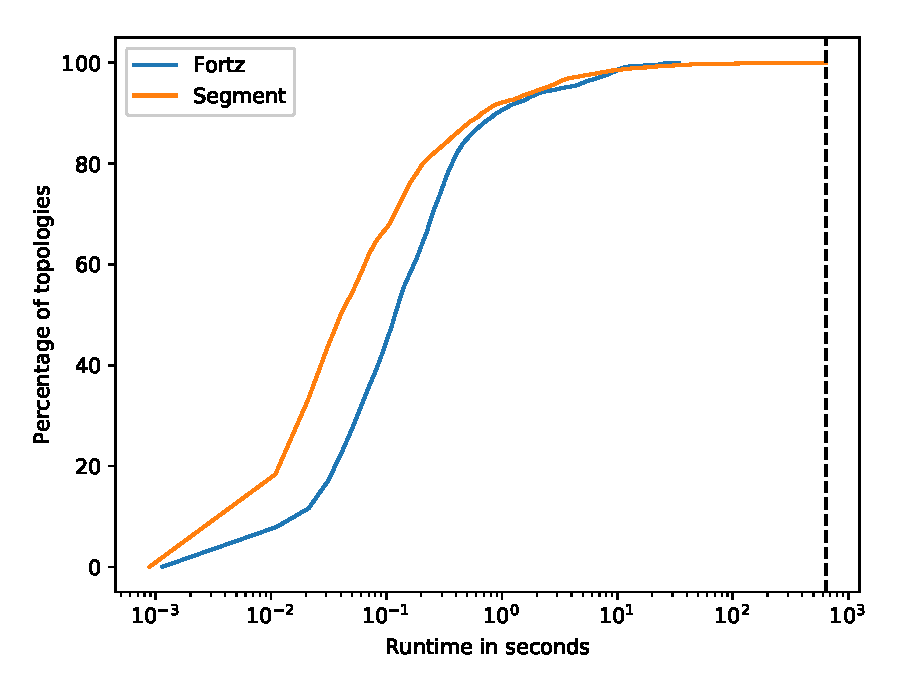
\includegraphics[width=.85\columnwidth]{./Network-lib/data/plot/maxEDPMip_runtime_both.eps}
\end{center}
\caption{CDF over all topologies of the runtime for solving $\sredpseg(G, s, t)$ and $\sredpfortz(G, s, t)$ over $100$ randomly selected source-destination pairs.}
\label{fig:maxEDP_runtime}
\end{figure}

\begin{figure}
\begin{center}
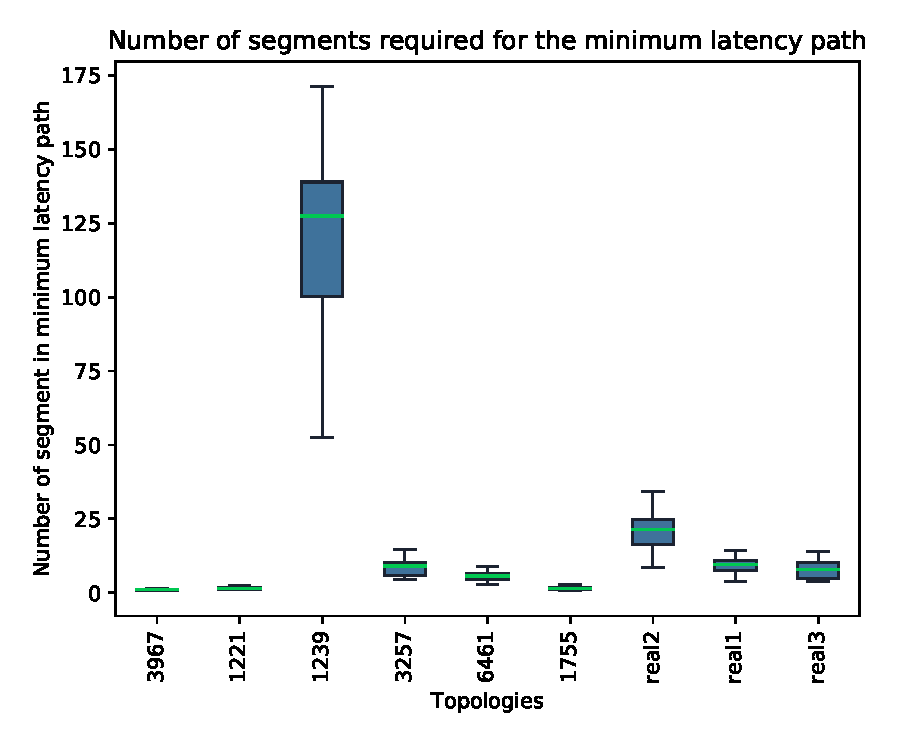
\includegraphics[width=.85\columnwidth]{./Network-lib/data/plot/maxEDP_boxplot.eps}
\end{center}
\caption{CDF over all topologies of the runtime for solving $\sredpfortz(G, s, t)$ over $100$ randomly selected source-destination pairs.}
\label{fig:maxEDP_boxplot}
\end{figure}

We also analyzed how restrictive the segmentation constraints with respect to the existence of disjoint paths.
For this we computed the difference between the maximum number of disjoint paths between the sources and the destinations
with the maximum number of disjoint sr-paths of segment cost at most $5$. Whenever this difference is $0$ we know that
requiring the path to be implementable with a segment cost of at most $5$ posed no restrictions in finding solutions.
Table \ref{tab:nbp_vs_seg} shows these results. We can see that for $95\%$ of the pairs the segmentation constraints were
not restrictive. This indicates that with about $5$ segments we can implement sets of sr-paths that are as large as the
theoretical maximum supported on the graph topology.

\begin{figure}
\begin{center}
\begin{tabular}{rccccc}
\toprule
difference & $0$ & $1$ & $2$ & $3$ & $\geq 4$ \\
\midrule
percentage of $s$-$t$           & 95\% & 4\% & 0.4\% & 0.1\% & 0.5\%
\end{tabular}
\end{center}
\caption{Percentage of pairs for each value of the difference between the maximum number of disjoint paths and maximum number of disjoint sr-paths with segment
cost at most $5$.}
\label{tab:nbp_vs_seg}
\end{figure}

\subsection{Minimizing the total latency}

For both models it is straightforward to modify the models to minimize the total latency of the sr-paths.
In both cases we need to first compute the maximum number of disjoint sr-paths that exist between the source
and destination, say $P$. Then, we need to replace the objective function by a minimization function that
adds all latencies together. We also need an additional constraint requiring the total number of paths in the solution to be equal to $P$.
Concretely, in the segment model, $\sredpseg(G, s, t)$, we can obtain this by replacing the objective function by
$$
\textbf{minimize} \quad \sum_{d = 1}^r \sum_{u \in V(G)} \sum_{v \in V(G)} \lat(u, v) \cdot x^d_{uv} 
$$
and adding a constraint
$$
\sum_{u \in V(G)} \sum_{d = 1}^r x^d_{su} = P. 
$$
For the Fortz model, $\sredpfortz(G, s, t)$, the change is analogous. The objective function
becomes 
$$
\textbf{minimize} \quad \sum_{i = 1}^k \sum_{u \in V(G)} \sum_{v \in V(G)} \lat(u, v) \cdot x^i_{uv} 
$$
and we add a constraint requesting $P$ paths starting at the source $s$:
$$
\sum_{u \in V(G)} x^1_{su} = P. 
$$

%\todo{Add plot comparing the runtime of minimizing latency vs not.}

\section{Min-max edge-disjoint sr-paths}

We now focus on the problem of computing pairs of disjoint paths with a min-max objective function. More
specifically, we aim at connecting via disjoint sr-paths a source node 
$s_1$ to a destination $t_1$ and a source node $s_2$ to a destination $t_2$
such that the maximum latency among those two paths is as small as possible.

\begin{problem}{Min-max edge-disjoint sr-paths}
\label{prob:disjointsrp}
\textbf{Input:} A network $G$ and $s_1, s_2, t_1, t_2 \in V(G)$ such that $s_1 \neq t_1$ and $s_2 \neq t_2$
and $k \in \mathbb{N}$.

\textbf{Output:} Two disjoint sr-paths $\sr{p}_1 \in \Pk(s_1, t_1), \sr{p}_2 \in \Pk(s_2, t_2)$ such that
$$
\max (\lat(\sr{p}_1), \lat(\sr{p}_2))
$$
is minimal.
\end{problem}

As we mentioned in the previous section, this problem is \NPhard \cite{minmax-disjoint-90, Li1990}.

\subsection{MIP formulation}

We saw above that Fortz model performed better than the segment model for computing maximal sets of disjoint paths.
However it is hard to enforce a source to destination assignment with this model. The reason is that different paths are not
modeled explicitly. For this reason, we use the segment model for solving Problem \ref{prob:disjointsrp}. With the segment model
each path is encoded in the index $d$ of the variables $x^d_{uv}$. This makes it easy to for the path starting at $s_1$ to end at $t_1$ and the
path starting at $s_2$ to end at $t_2$. The adapted model is the following.

\begin{center}
\begin{tabular}{rcllr}
\multicolumn{5}{l}{$\sredp(G, s_1, s_2, t_1, t_2)$} \\[0.5cm] 
\multicolumn{3}{l}{$\mathbf{min} \quad \lambda$} & $\textbf{s.t.}$ & \\[0.5cm]
$\displaystyle \sum_{d = 1}^2 \sum_{u \in V(G)} \sum_{v \in V(G)}  x^d_{uv} \cdot I(u, v, e)$ & $\leq$ & $1$ & $\forall e \in E(G)$ & \\[0.5cm]
$\displaystyle \sum_{u \in V(G) \setminus \{ v \}} x^d_{uv} - \sum_{u \in V(G) \setminus \{ v \}} x^d_{vu}$ & $=$    &  $0$ & $\forall d \in \{1,2\}$, $\forall v \in V(G) \setminus \{ s_d, t_d \}$ & \\[0.5cm]
$\displaystyle \sum_{u \in V(G)} \sum_{v \in V(G)} \lat(u, v) \cdot x^d_{u, v}$ & $\leq$    & $\lambda$ & $\forall d \in \{ 1, 2 \}$ \\[0.5cm]
$\displaystyle \sum_{u \in V(G) \setminus \{ s_d \}} x^d_{s_d u}$ & $=$    & $1$ & $\forall d \in \{ 1, 2 \}$ \\[0.5cm]
$\displaystyle \sum_{u \in V(G) \setminus \{ t_d \}} x^d_{u t_d}$ & $=$    & $1$ & $\forall d \in \{ 1, 2 \}$ \\[0.5cm]
$\displaystyle \sum_{d = 1}^2 \sum_{u \in V(G)} x^d_{u s_d} +  x^d_{t_d u}$ & $=$    & $0$ & $\forall d \in \{ 1, 2 \}$ \\[0.5cm]
$\displaystyle \sum_{u \in V(G)} \sum_{v \in V(G)} x^d_{uu}$ & $\leq$      & $k$ & $\forall d \in \{ 1, 2 \}$ \\[0.5cm]
$x^d_{uv}$  &    $\in$    &  $\{0, 1\}$  & $\forall e \in E(G), \ \forall d \in \{1, 2 \}$ & \\[0.5cm]
$\lambda$   &    $\geq$   & $0$ & &
\end{tabular}
\end{center}


\subsection{Dedicated algorithm}

We also proposed a dedicated algorithm for solving this problem. This was actually our original idea that was published in CoNEXT 18 \cite{rdp}.
However we will see that it is actually less efficient and flexible than the MIP formulation.
Recall that in our definition of network, we mentioned that each edge is indexed with a unique number between $0$ and $|E(G)| - 1$. This is useful for
defining parallel edges. These indexes are also important in the context of disjoint paths. From an implementation point of view, we will represent the
set of edges corresponding to a sr-path $\sr{p}$, $E(\sr{p})$, as a \emph{bitset} $b$ such that $b_i = 1$ if and only if edge with $\idx(e) = i$ belongs
to $E(\sr{p})$.

Bitsets are a very simple and efficient way to represent subsets of $\{ 0, \ldots, n - 1 \}$ for some fixed, not too large value of $n$. Conceptually they
are similar to an array of booleans of size $n$. However, a bitset is represented instead (on a 64-bit machine) with an array of \texttt{long}. Each element of the array
represents a group of $64$ boolean values with its bits. So the bits of the first element in the array will represent elements $0$ to $63$, the second $64$ to $127$ and 
so forth. Figure \ref{fig:bitset} illustrates a bitset for $n = 512$. In this example, element $131$ is represented by the forth bit of
the third long.

\begin{figure}
\begin{center}
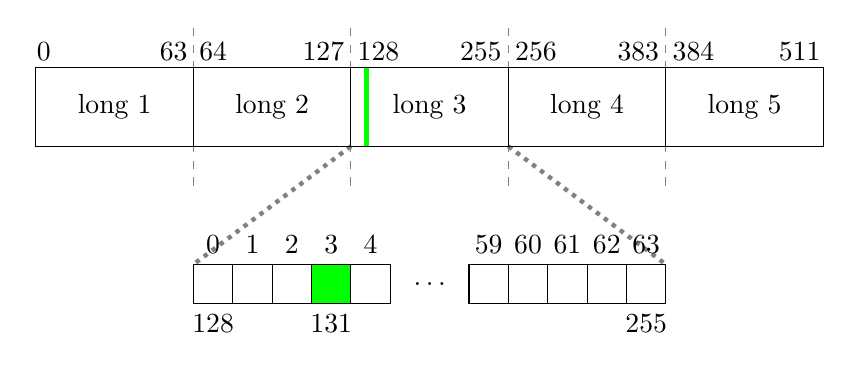
\begin{tikzpicture}

\draw[green, ultra thick] (4.2, 0) -- (4.2, 1);


\draw[dashed, gray] (2, -0.5) -- (2, 1.5);
\draw[dashed, gray] (4, -0.5) -- (4, 1.5);
\draw[dashed, gray] (6, -0.5) -- (6, 1.5);
\draw[dashed, gray] (8, -0.5) -- (8, 1.5);

\fill[green] (3.5, -2) rectangle (4, -1.5);

\draw[gray, ultra thick, dotted] (4, 0) -- (2, -1.5);
\draw[gray, ultra thick, dotted] (6, 0) -- (8, -1.5);

\draw[step=2] (0, 0) grid (10, 1);
\draw (0, 0) rectangle (10, 1);

\draw[step=0.5] (2, -2) grid (4.5, -1.5);
\draw (2, -2) rectangle (4.5, -1.5);

\draw[step=0.5] (5.5, -2) grid (8, -1.5);
\draw (5.5, -2) rectangle (8, -1.5);

\node at (5, -1.75) {$\ldots$};

\node at (2.25, -1.25) {0};
\node at (2.75, -1.25) {1};
\node at (3.25, -1.25) {2};
\node at (3.75, -1.25) {3};
\node at (4.25, -1.25) {4};


\node at (2.25, -2.25) {128};
\node at (2.25 + 1.5, -2.25) {131};

\node at (5.5 + 2.25, -2.25) {255};

\node at (5.5 + 0.25, -1.25) {59};
\node at (5.5 + 0.75, -1.25) {60};
\node at (5.5 + 1.25, -1.25) {61};
\node at (5.5 + 1.75, -1.25) {62};
\node at (5.5 + 2.25, -1.25) {63};

\node at (0.1, 1.2) {0};
\node at (1.75, 1.2) {63};

\node at (2.25, 1.2) {64};
\node at (3.65, 1.2) {127};

\node at (4.35, 1.2) {128};
\node at (5.65, 1.2)  {255};

\node at (6.35, 1.2) {256};
\node at (7.65, 1.2) {383};

\node at (8.35, 1.2) {384};
\node at (9.7, 1.2) {511};

\node at (1, 0.5) {long 1};
\node at (3, 0.5) {long 2};
\node at (5, 0.5) {long 3};
\node at (7, 0.5) {long 4};
\node at (9, 0.5) {long 5};

\end{tikzpicture}
\end{center}
\caption{Representation of a bitset with $n = 512$.}
\label{fig:bitset}
\end{figure}

The advantage of this representation over a boolean array representation is that each set operation on a long can be performed in $O(1)$.
So for example, to compute the intersection between two bitsets we simply need to loop over the array and perform a bitwise and between
corresponding elements. Therefore we only need to perform $n \slash 64$ operations rather $n$. Even though in big-Oh notation this sill yields
the same complexity, $O(n)$, the runtime in practice is $64$ times faster which is a gigantic speedup.
Using a bitset representation for the set of edges of a sr-path we can then perform set operations over these very efficiently. 

In particular, this representation makes it possible to very efficiently check whether or not two sr-paths are disjoint. We exploit this to
design an algorithm for solving \ref{prob:disjointsrp}. Given a sr-path $\sr{p}_1$ we can find the minimum latency sr-path $\sr{p}_2$ that
is disjoint from it in polynomial time by using the minimum latency sr-path algorithm from Chapter \ref{chapter:sr-optimal}. We simply need to
adapt it so that it avoids $E(\sr{p}_1)$. To do so, we need to know the set of edges in all sr-paths of the form $\langle x, y \rangle$
where $x, y \in V(G)$. We show how to do this in the next.

\subsubsection{Pre-computing the forwarding graphs}

\begin{lemma}
\label{lemma:forwdp}
Let $G$ be a network and $x, y \in V(G)$. Then
\begin{equation}
\label{eq:forwdp}
E(\sp(x, y)) = \bigcup_{ e \in \ine(\sp(x), y) } E(\sp(x, e^1)) \cup \{ e \}.
\end{equation}
\end{lemma}

\begin{proof}
$(\subseteq)$ Let $e \in E(\sp(x, y))$. Let $p = (e_1, \ldots, e_n)$ be a shortest path from $x$ to $y$ 
passing by $e$. Then $e = e_i$ for some $i$.  Note that $(e_1, \ldots, e_{n - 1})$ 
is a shortest path from $x$ to $e^2_{n - 1} = e^1_n$ and, since $e^2_n = y$, 
$e_n \in \ine(\sp(x), y)$. Thus, if $i = n$ then $e$ clearly belongs to the right-hand
side of (\ref{eq:forwdp}). Otherwise, if $i < n$ then $e$ belongs to the shortest 
path $(e_1, \ldots, e_{n - 1})$ from $x$ to $e^2_{n - 1} = e^1_n$. Since $e_n \in
\ine(\sp(x), y))$ we again conclude that $e$ belongs to the rhs of (\ref{eq:forwdp}).

$(\supseteq)$ Let $e$ be a edge belonging to the rhs of (\ref{eq:forwdp}). There exists
$f \in \ine(\sp(x), y))$ such that either $e = f$ or $e \in E(\sp(x, f^1))$. If $e = f$
then $e = f \in \ine(\sp(x), y)) = \ine(\sp(x, y))$ so it belongs to $\sp(x, y)$. Otherwise,
$e$ belongs to a shortest path from $x$ to the origin of $f$. Since $f \in \ine(\sp(x), y)$
we have that $\dist(x, y) = \dist(x, f^1) + \igp(f)$. Since $e$ belongs to a shortest
path $p$ from $x$ to $f^1$, we have 
$\dist(x, e^1) + \igp(e) + \dist(e^2, f^1) = \dist(x, f^1) = \igp(p)$.
Then
\begin{align*}
\dist(x, y) & = \dist(x, f^1) + \igp(f) \\
& = \dist(x, e^1) + \igp(e) + \dist(e^2, f^1) + \igp(f) \\
& = \dist(x, e^1) + \igp(e) + \dist(e^2, f^2) \\
& = \dist(x, e^1) + \igp(e) + \dist(e^2, y) \\
\end{align*}
so that $e \in \sp(x, y)$.
\end{proof}

Using Lemma \ref{lemma:forwdp} we can leverage the speed of bitsets to
efficiently compute $E(\SP(v, u))$ for all $u, v \in V(G)$. Note that we
could always compute them using the definition, that is, computing 
$\sp(u)$ for all $u$ and then for each $v$ using a breath-first search to
extract the subset of edges of $\sp(u)$ that belong to $\sp(u, v)$. 
Using equation (\ref{eq:forwdp}), we can compute $E(\sp(u, v))$ by
performing $|\ine(\sp(u), v)|$ bitset operations. As we mentioned above,
in theory this is not faster but it practice it runs faster even due to the
usage of bitsets. However, in the next section we will see that applying the same idea
to precompute another kind of data that we will need leads to huge gains in
runtime. Algorithm \ref{algo:preforw} shows how we can easily compute this recurrence.
For each $u$ we compute the shortest path subnetwork rooted at $u$ and then compute
a topological order $v_1, v_2, \ldots, v_n$ to compute $E(\sp(u, v_i)$ in an order such
that when computing $E(\sp(u, v_i))$ we already computed $E(\sp(u, e^1))$ for all $e \in
\ine(\sp(u), v_i)$.

%as shown in Figure \ref{fig:precompute_forw_runtime}.

%\begin{figure}
%\begin{center}
%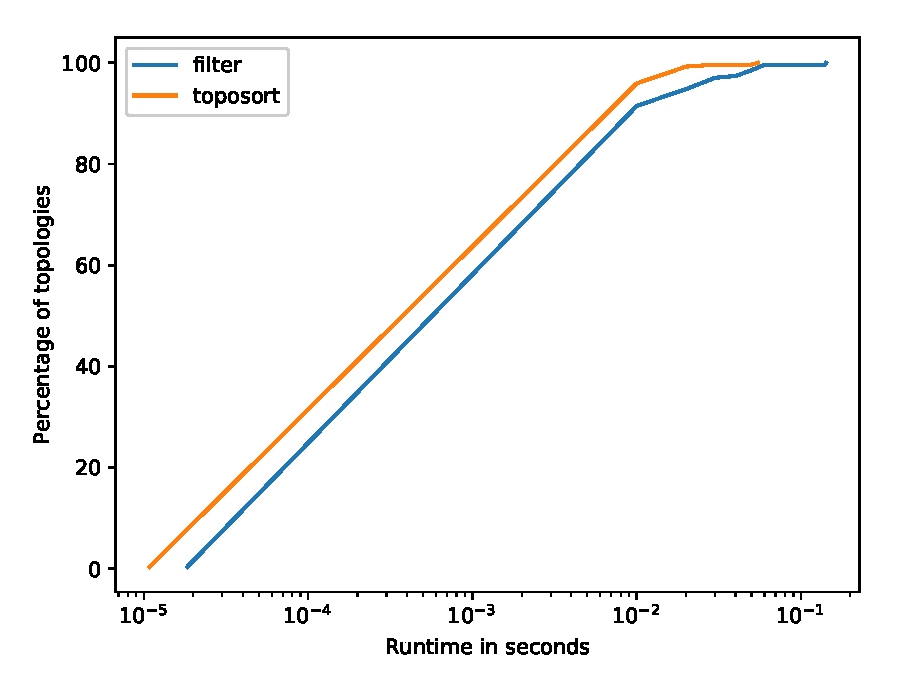
\includegraphics[width=.85\columnwidth]{./Network-lib/data/plot/precompute_forw_runtime.eps}
%\end{center}
%\caption{todo}
%\label{fig:precompute_forw_runtime}
%\end{figure}

\begin{algorithm}[t]
\small
\caption{$\textsf{precompute-forwEdges}\left( g \right)$}
\begin{algorithmic}[1]
\FOR{$u, v \in V(G)$}
  \STATE $fwe(u, v) \gets \textsf{Bitset}()$
\ENDFOR
\FOR{$u \in V(G)$}
  \STATE $\sp(u) \gets \textsf{dikstra-dag}(g, u)$
  \STATE $order \gets \textsf{toposort}(\sp(u))$
  \FOR{$v \in order$}
    \FOR{$e \in \ine(\sp(u), v)$}
      \STATE $fwe(u, v) \gets fwe(u, e^1) \cup \{ e \}$
    \ENDFOR
  \ENDFOR
\ENDFOR
\RETURN $fwe$
\end{algorithmic}
\label{algo:preforw}
\end{algorithm}

Having pre-computed $E(\sp(u, v))$ we can easily adapt Algorithm
\ref{algo:min_weight_sr_path} to make sure that the path that is computed avoids all
edges in $E(\sr{p}_1)$. Recall that, according to Chapter \ref{chapter:sr-optimal}, 
the recurrence for the minimum latency path
from $s_2$ to $v$ with segment cost at most $i$ will be

\[\mathit{sol}(i, v) = \min \left\{
  \begin{matrix}
    \mathit{sol}(i - 1, v) &  \\[0.2cm]
    \mathit{sol}(i - 1, u)  +  \lat(u, v)  & \textbf{s.t} \text{ $u \in V$} \\[0.2cm]
    \mathit{sol}(i - 2, r)  +  \lat(r, e^1) + \lat(e) & \textbf{s.t} \text{ $u \in V, e \in \ine(v)$} \\
\end{matrix}
  \right.
\]

as illustrated by Figure \ref{fig:dp_disjoint}. In order to guarantee disjointness,
we just need to ensure that for each case all pieces are disjoint
from $\sr{p}_1$. This means ensuring that 
$$
E(\sp(u, v)) \cap E(\sr{p}_1) = \emptyset
$$
in the second case and that 
$$\left( E(\sp(u, e^1)) \cup \{ e \} \right) \cap E(\sr{p}_1) = \emptyset
$$
in the third case. In term of algorithms, this corresponds to adding these conditions
to lines \ref{mwsrp-if1} and \ref{mwsrp-if2} from Algorithm \ref{algo:min_weight_sr_path}, respectively. Note that these changes will
have a minor impact over the overall performance of the algorithm since we use bitsets
to compute these intersections and $E(\sp(u, v))$ is given as input for all $u, v \in V(G)$.

 \begin{figure}
 \begin{center}
 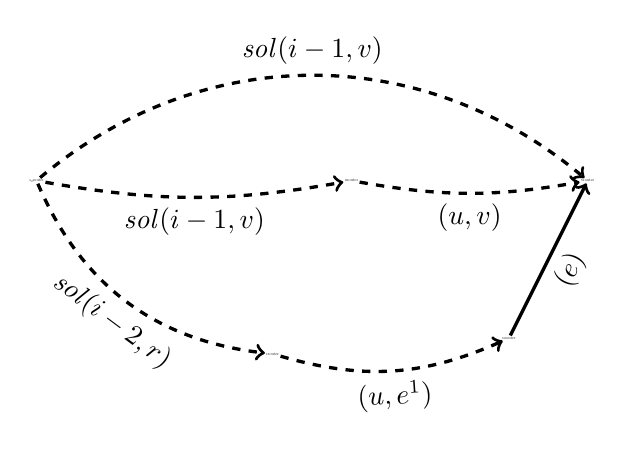
\begin{tikzpicture}
 \node[scale=0.15] (s) at (0, 0) {\router{$s_2$}{router}};
 \node[scale=0.15] (x) at (5+2, 0) {\router{v}{router}};
 \node[scale=0.15] (y) at (2+2, 0) {\router{u}{router}};
 \node[scale=0.15] (z) at (4+2, -2) {\router{u}{router}};
 \node[scale=0.15] (r) at (2+1, -2-0.2) {\router{r}{router}};
 
 
 
 \draw (s) edge[very thick, below, bend right=10, dashed, ->] node {$\mathit{sol}(i - 1, v)$} (y);
 \draw (y) edge[very thick, bend right=10, dashed, ->, below] node {$\lat(u, v)$} (x);
 \draw (s) edge[very thick, bend left=40, dashed, ->, above] node {$\mathit{sol}(i - 1, v)$} (x);
 %\draw (s) edge[very thick, bend right=30, dashed, ->] (z);
 \draw (z) edge[very thick, ->, sloped, below] node {$\lat(e)$} (x);
 
 \draw (s) edge[very thick, bend right=30, dashed, ->, below, sloped] node {$\mathit{sol}(i - 2, r)$} (r);
 \draw (r) edge[very thick, bend right=20, dashed, ->, below, sloped] node {$\lat(u, e^1)$} (z);
 
 \end{tikzpicture}
 \end{center}
 \caption{Illustration of the $\mathit{sol}$ recurrence}
 \label{fig:dp_disjoint}
 \end{figure}

In order to find a pair of paths, we perform a depth-first search on $\sr{p}_1$ and use
the above algorithm to maintain the minimum latency sr-path $\sr{p}_2$ that is disjoint from the 
current partial path $\sr{p}_1$. At each step of the search, we try to extend $\sr{p}_1$
with either a node segment or an adjacency segment. We perform the following steps to
avoid exploring useless extensions of $\sr{p}_1$. Let $\sr{p}_1 = \langle
x_1, \ldots, x_n \rangle$ be the partial path at given search node, $\sr{p}_2$
the minimum latency sr-path disjoint from the partial path $\sr{p}_1$, $l^*$ the 
latency of the best solution found so far and $x$ be a node or adjacency segment:

\begin{itemize}
 \item Let $v = x^2_n$ be the node where $\sr{p}_1$ ends. In the best case, the latency
 of the completed sr-path $\sr{p}_1$ will be its current latency plus the latency of the minimum
 latency path between $v$ and $t_1$ in $G$. Let's denote that latency by $\mathcal{L}(v, t_1)$.
 Therefore, if $\max(\lat(\sr{p}_1) + \mathcal{L}(v, t_1), \lat(\sr{p}_2)) \geq l^*$
 we can stop the search since we will never reach a better solution.
 
 \item By Theorem \ref{thm:sracyclic}, there is
 a solution to Problem \ref{prob:disjointsrp} where both $\sr{p}_1$ and $\sr{p}_2$ are acyclic.
 Hence, we can ignore $x$ if $\sr{p}_1 \oplus x$ is cyclic. Checking this can be 
 done efficiently thanks to our bitset representation and forwarding graph
 edge set pre-computation.
 
 \item If $\sr{p}_1 \oplus x$ does not intersect 
 $\sr{p}_2$ then $\sr{p}_2$ remains the minimum latency sr-path that is disjoint from
 $\sr{p}_1 \oplus x$ so there is not need to re-compute it. Otherwise, we use the algorithm
 that we described above to compute a new minimum latency sr-path $\sr{p}_2$. If this path does
 not exist, then it is fruitless to try $x$ as an extension of $\sr{p}_1$.
 
 \item If there does not exist a pair of disjoint paths
 on $G$, one from $x^2$ to $t_1$ and another from $s_2$ to $t_2$ then we will never reach a 
 solution by extending $\sr{p}_1$ with $x$. However, we have seen that checking whether
 such disjoint paths exists is \NPcomplete. We use a relaxation of this condition by allowing
 the path from $x^2$ to go to $t_2$ or the path from $s_2$ to go to $t_1$ which is equivalent
 to checking whether the maximum flow between $\{x^2, s_2\}$ and $\{t_1, t_2\}$ is
 at least $2$.
\end{itemize}

By putting all these ideas together we can formally express Algorithm
\ref{algo:disjoint_srp} and \ref{algo:disjoint_srp_dfs} for solving Problem
\ref{prob:disjointsrp}.

\begin{algorithm}[t]
\small
\caption{$\textsf{disjoint-srpaths}\left( g, s_1, s_2, t_1, t_2 \right)$}
\begin{algorithmic}[1]
\STATE $\sr{p}_2 \gets \textsf{min-lat-disjoint-srpath}(s_2, t_2, k)$
\STATE $l^* \gets \infty$
\FOR{$x \in V(G) \cup E(g)$}
  \STATE $\textsf{disjoint-srpaths-dfs}\left( \langle x \rangle, \sr{p}_2 \right)$
\ENDFOR
\IF{$l^* = \infty$}
  \RETURN \textbf{null}
\ENDIF
\RETURN $\sr{p}^*_1, \sr{p}^*_2$
\end{algorithmic}
\label{algo:disjoint_srp}
\end{algorithm}

\begin{algorithm}[t]
\small
\caption{$\textsf{disjoint-srpaths-dfs}\left( \sr{p}_1, \sr{p}_2 \right)$}
\begin{algorithmic}[1]
\IF{$\max(\lat(\sr{p}_1) + \mathcal{L}(\sr{p}_1.\textsf{dest}(), t_1) \geq l^*$} 
  \RETURN
\ENDIF
\cmtline{we reached here so if the path is complete, it is a better solution}
\IF{$\sr{p}_1.\textsf{dest}() = t_1$}
  \STATE $l^* \gets \max(\lat(\sr{p}_1), \lat(\sr{p}_2))$
  \STATE $\sr{p}^*_1, \sr{p}^*_2 \gets \sr{p}_1, \sr{p}_2$
  \RETURN
\ENDIF
\cmtline{try extend $\sr{p}_1$ with a node segment}
\IF{$\cost(\sr{p}_1) + 1 > k$}
  \RETURN
\ENDIF
\FOR{$u \in V(G)$}
  \cmtline{check whether we can cut with min cost flow}
  \STATE $P, l \gets \textsf{min-cost-flow}(g, \{u, s_2\}, \{t_1, t_2\})$
  \IF{$|P| < 2 \textbf{ or } l \geq l^*$}
    \RETURN
  \ENDIF
  \cmtline{check whether adding $u$ will keep $\sr{p}_1$ acyclic}
  \IF{$E(\sp(\sr{p}_1.\textsf{dest}(), u)) \cap E(\sr{p}_1) = \emptyset$}
    \RETURN
  \ENDIF
  \STATE $\sr{p}_1.\textsf{addLast}(u)$
  \IF{$E(\sr{p}_1) \cap E(\sr{p}_2) = \emptyset$}
    \STATE $\textsf{disjoint-srpaths-dfs}\left( \sr{p}_1, \sr{p}_2 \right)$
  \ELSE
    \STATE $\sr{p}'_2 \gets \textsf{min-lat-disjoint-srpath}(\sr{p}_1, s_2, t_2, k)$
    \IF{$\sr{p}'_2 \neq \textbf{null}$}
      \STATE $\textsf{disjoint-srpaths-dfs}\left( \sr{p}_1, \sr{p}'_2 \right)$
    \ENDIF
  \ENDIF
  \STATE $\sr{p}_1.\textsf{removeLast}()$
\ENDFOR
\cmtline{try extend $\sr{p}_1$ with an adjacency segment}
\IF{$\cost(\sr{p}_1) + 2 > k$}
  \RETURN
\ENDIF
\FOR{$e \in E(g)$}
  \cmtline{check whether we can cut with min cost flow}
  \STATE $P, l \gets \textsf{min-cost-flow}(g, \{e^2, s_2\}, \{t_1, t_2\})$
  \IF{$|P| < 2 \textbf{ or } l \geq l^*$}
    \RETURN
  \ENDIF
  \IF{$\left( E(\sp(\sr{p}_1.\textsf{dest}(), e^1)) \cup \{e\} \right) \cap E(\sr{p}_1) \neq \emptyset$}
    \RETURN
  \ENDIF
  \cmtline{check whether adding $e$ will keep $\sr{p}_1$ acyclic}
  \STATE $\sr{p}_1.\textsf{addLast}(e)$
  \IF{$E(\sr{p}_1) \cap E(\sr{p}_2) = \emptyset$}
    \STATE $\textsf{disjoint-srpaths-dfs}\left( \sr{p}_1, \sr{p}_2 \right)$
  \ELSE
    \STATE $\sr{p}'_2 \gets \textsf{min-lat-disjoint-srpath}(\sr{p}_1, s_2, t_2, k)$
    \IF{$\sr{p}'_2 \neq \textbf{null}$}
      \STATE $\textsf{disjoint-srpaths-dfs}\left( \sr{p}_1, \sr{p}'_2 \right)$
    \ENDIF
  \ENDIF
\ENDFOR
\end{algorithmic}
\label{algo:disjoint_srp_dfs}
\end{algorithm}

\subsubsection{Algorithm comparison}

We compared both algorithms in terms of runtime. For this, we generated $100$ tuples
$(s_1, s_2, t_1, t_2)$ and computed disjoint sr-path using the MIP algorithm and the dedicated
algorithm for $k = 3$ and $k = 4$. Figure \ref{fig:perf3} shows the performance profile of the algorithms for $k = 3$.
A performance profile shows the CDF of the ratio of the runtime of each algorithm and the minimum runtime amongst the two.
We can observe that the MIP model is faster for $64\%$ of the tuples. The MIP model is at most
$20$ times slower whereas the dedicated algorithm can be up to $53$ times slower. This 
indicates that MIP model is more efficient than the dedicated algorithm. This gets
even more evident as we grow $k$. For $k = 4$, as shown in Figure \ref{fig:perf4},
the MIP model performs much better than the dedicated algorithm. It is faster for $80\%$
of the tuples and when it is not, it is barely slower.

\begin{figure}
\begin{center}
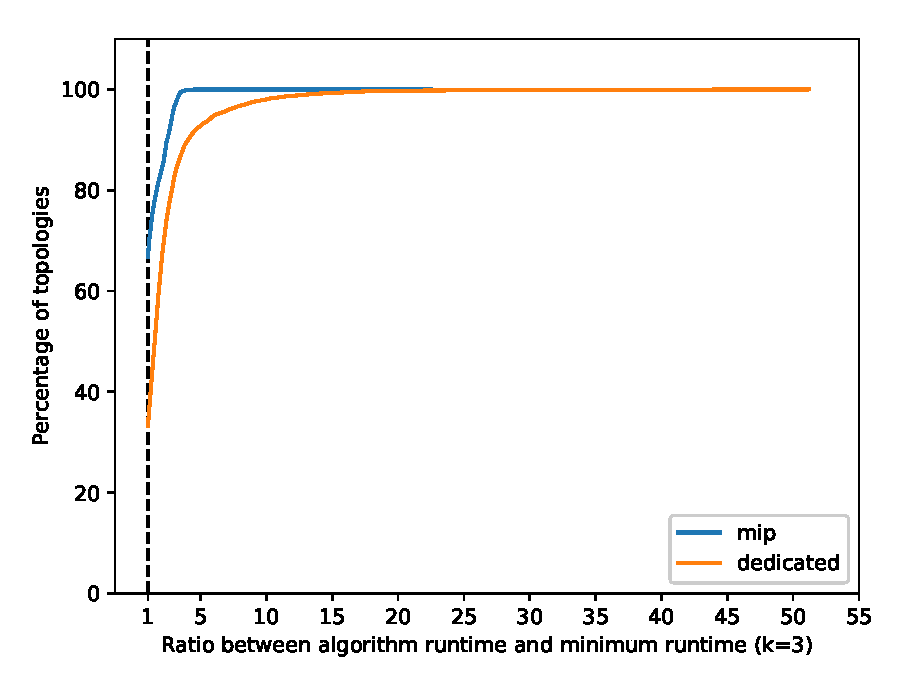
\includegraphics[width=.85\columnwidth]{./Network-lib/data/plot/2SREDP_3.eps}
\end{center}
\caption{Performance profile between the MIP model and the dedicated algorithm for $k = 3$.}
\label{fig:perf3}
\end{figure}

\begin{figure}
\begin{center}
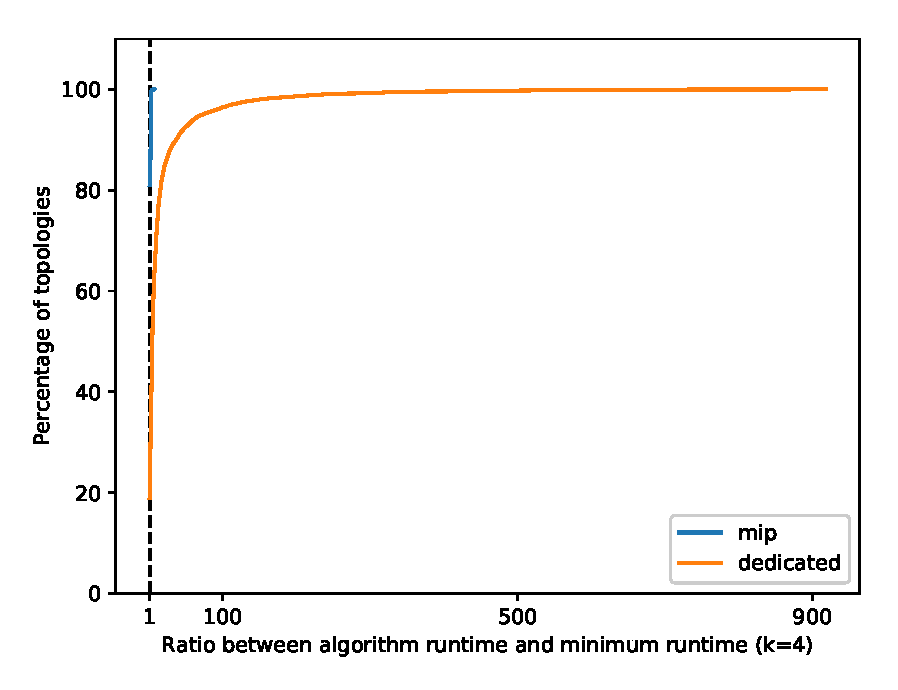
\includegraphics[width=.85\columnwidth]{./Network-lib/data/plot/2SREDP_4.eps}
\end{center}
\caption{Performance profile between the MIP model and the dedicated algorithm for $k = 4$.}
\label{fig:perf4}
\end{figure}





\section{Robustly disjoint sr-paths}
\label{section:rdp}

In this section we propose a technique to leverage segment routing to provide a failure
tolerant disjoint path service. The idea is to connect two sites via a pair of 
disjoint sr-paths like we did in the previous section and ensure these sites remain connected by two disjoint paths
even in case of a link failures. Segment routing is interesting in such
a setting because, since it is based on shortest path routing, after a set
of network links goes down, these sr-paths will automatically converge towards new paths on $G$
as the routers update theirs routing tables. 

The idea is thus to take this into account when building the sr-paths and 
make sure that the set of paths on $G$ that correspond the sr-paths are disjoint
after IGP re-convergence for any given failure. If we manage to compute such paths, then we have the guarantee
that our solution remains disjoint even in case something goes wrong.

Concretely, we will assume that a set of failure that we want to support is
given as input and we will seek pairs of paths that are tolerant to any 
failure in the given set.

\begin{definition}
Let $G$ be a network. A \emph{failure set} is a set $F = \{f_1, \ldots, f_m\}$ such that
for all $i$, $f_i \subseteq E(G)$ and $\emptyset \in F$.
\end{definition}

Requiring that the empty set belongs to the failure sets poses no practical restriction
and is there just to make the following definitions more elegant.

If we want to support single link failures we can set $F = \{ \{ e \} \mid e \in E(G) \} \cup \{ \emptyset \} = F_E(G)$.
If we know specific shared risk link groups~\cite{ghobadi-imc16,turner2010california} we can also add
them to $F$ so that our paths become failure tolerant to them.
Note that there are limits to the amount of failures that one can add to $F$. If we add too many
failure sets then we have a high chance of over constraining the problem and making it have no
admissible solution.

We model a failure of a set of edges $f \in F$ as removing those edges from the network. Therefore
it can happen that the network becomes disconnected after a failure occurs. This can lead to the fact
that the sr-paths might become undefined if they either require to route traffic between disconnected parts of the network
or they use an adjacency segment over an element of $f$. In particular, this means that we cannot use adjacency segments
over any link belonging to an edge in $F$ since such a failure would make the path unusable. As a consequence,
if $F = F_E(G)$ then we cannot use adjacency segments at all. This leads to the following definition.

%For this reason,
%we will simply ignore adjacency segments in this section and consider only paths with node segments only.

\begin{definition}
Let $G$ be a network, $\sr{p} = \langle x_1, \ldots, x_n \rangle$ a sr-path on $G$ and $F$ a failure set. We say that $\sr{p}$ is \emph{well defined
with respect to $F$} if $\sr{p}$ does not contain any adjacency segment belonging to a set $f \in F$
and for each $i = 2, \ldots, n$ and $f \in F$, $G \setminus f$ contains at least one path from $x^2_{i - 1}$ to $x^1_i$.
\end{definition}

Figure \ref{fig:welldefined} illustrates this definition. Suppose that the failure set $F$ contains a failure set $f$ whose
elements consist of all edges touching node $\node{i}$ (in both directions). Then any path using node $\node{i}$ as a segment
will not be well defined with respect to $F$. For instance, $\sr{p} = \langle \node{a}, \node{g}, \node{i}, \node{h} \rangle$
will fail to forward packets from $\node{g}$ to $\node{i}$ if failure $f$ occurs.
This example also illustrates another important aspect of robustly disjoint paths. Imagine that we want to consider node failures
and also have disjoint sr-paths that are tolerant to node failures. We can model a node failure with a failure set $f$ consisting
of all edges incident to that node (in both directions). However, this will imply that that node becomes a forbidden node segment for
any sr-path in the solution. A corollary of this is that it is impossible to have robustly disjoint paths that are tolerant to the failure of
\emph{any} node since this would prevent any sr-path to contain segments altogether.

\begin{figure}
\begin{center}
\begin{tikzpicture}
\def\x{0}
\def\y{0}

\node[scale=0.15] (a) at (0.5 + \x,  0.5 + \y) {\router{a}{marked}};
\node[scale=0.15] (b) at (0.5 + \x, -1.0 + \y) {\router{b}{router}};
\node[scale=0.15] (c) at (2.5 + \x,  0.0 + \y) {\router{c}{router}};
\node[scale=0.15] (d) at (4.5 + \x,  0.0 + \y) {\router{d}{router}};
\node[scale=0.15] (e) at (4.0 + \x, -2.0 + \y) {\router{e}{router}};
\node[scale=0.15] (g) at (6.0 + \x,  0.5 + \y) {\router{g}{marked}};
\node[scale=0.15] (i) at (8.0 + \x,  0.0 + \y) {\router{i}{marked}};
\node[scale=0.15] (h) at (7.0 + \x, -1.5 + \y) {\router{h}{marked}};
\node[scale=0.15] (f) at (4.0 + \x, -3.5 + \y) {\router{f}{router}};
\node[scale=0.15] (j) at (8.0 + \x, -2.5 + \y) {\router{j}{router}};
\draw[line width=2] (a) edge[above, sloped] node[black] {} (b);
\draw[line width=2]  (a) edge[above, sloped] node[black] {} (c);

\draw[line width=2] (b) edge[above, sloped] node[black] {} (c);
\draw[line width=2] (b) edge[above, sloped] node[black] {} (e);
\draw[line width=2] (b) edge[above, sloped] node[black] {} (f);
\draw[line width=2]  (c) edge[above, sloped] node[black] {} (d);
\draw[line width=2]  (d) edge[above, sloped] node[black] {} (e);
\draw[line width=2]  (d) edge[above, sloped] node[black] {} (g);
\draw[line width=2] (e) edge[above, sloped] node[black] {} (c);
\draw[line width=2] (e) edge[above, sloped] node[black] {} (f);
\draw[line width=2] (f) edge[above, sloped] node[black] {} (j);
\draw[line width=2] (f) edge[above, sloped] node[black] {} (h);
\draw[line width=2, red] (g) edge[above, sloped] node[black] {} (i);
\draw[line width=2]  (g) edge[above, sloped] node[black] {} (h);
\draw[line width=2] (h) edge[above, sloped] node[black] {} (j);
\draw[line width=2, red] (i) edge[above, sloped] node[black] {} (h);
\draw[line width=2]  (e) edge[above, sloped] node[black] {} (h);

\draw[line width=3, darkgreen]  (a) edge[above, bend left=15, sloped, ->] node[black] {} (c);
\draw[line width=3, darkgreen]  (c) edge[above, bend left=15, sloped, ->] node[black] {} (d);
\draw[line width=3, darkgreen]  (d) edge[above, bend left=15, sloped, ->] node[black] {} (g);
\draw[line width=3, darkgreen]  (g) edge[above, bend left=15, sloped, ->] node[black] {} (i);
\draw[line width=3, darkgreen]  (i) edge[above, bend left=15, sloped, ->] node[black] {} (h);

\node[draw, fill=green!50!white, above = 0.1cm of a] (y1) {\small $x_1$};
\node[draw, fill=green!50!white, above = 0.1cm of g] (y2) {\small $x_2$};
\node[draw, fill=green!50!white, above = 0.1cm of i] (y3) {\small $x_3$};
\node[draw, fill=green!50!white, right = 0.1cm of h] (y3) {\small $x_4$};

\end{tikzpicture}
\end{center}
\caption{The sr-path $\langle \node{a}, \node{g}, \node{i}, \node{h} \rangle$ is not well defined if edges 
$\edge{g}{i}$, $\edge{i}{g}$, $\edge{i}{h}$, $\edge{h}{i}$ are in $F$.}
\label{fig:welldefined}
\end{figure}


We can now define the robustly disjoint paths (RDPs).

\begin{definition}
Let $G$ be a network, $\sr{p}_1$, $\sr{p}_2$ be two sr-paths and $F$ a failure set. We say that
$\sr{p}_1$ and $\sr{p}_2$ are \emph{robustly disjoint} if they are disjoint and well defined
on $G \setminus f$ for every $f \in F$.
\end{definition}

You can see that this definition also ensures that robuslty disjoint paths are 
disjoint to begin with since we assume that $\emptyset \in F$.

\begin{problem}{Robustly disjoint sr-path problem}
\label{prob:rdp}
\textbf{Input:} A network $G$, a failure set $F$, $s_1, s_2, t_1, t_2 \in V(G)$ and $k \in \mathbb{N}$.

\textbf{Output:} Two robustly disjoint sr-paths $\sr{p}_1 \in \Pk(s_1, t_1)$, $\sr{p}_2 \in \Pk(s_2, t_2)$ with respect to $F$.
\end{problem}

Since Problem \ref{prob:disjointsrp} is \NPhard, this problem must also be since we get the same problem
by setting $F = \{ \emptyset \}$.

It is not hard to adapt the disjoint sr-path MIP model proposed in the previous section 
to the case of robustly disjoint paths as well as our dedicated algorithm as we will show in the
remainder of this section.

\subsection{Adapting $\sredp$ to RDPs}

Adapting model $\sredp(G, s_1, s_2, t_1, t_2)$ to support robustly disjoint paths
is very simple. The only thing that we need to change are the disjointness constraints
so that they take the failures into account.

Recall that we ensure disjointness by requiting that if $e \in E(\sp(u, v))$ then
at most one of $x^1_{uv}, x^2_{uv}$ is set to $1$. To ensure that the sr-paths 
are robuslty disjoint we need to ensure that if
$$
e \in \bigcup_{f \in F} E(\sp(G \setminus f, u, v))
$$
then at most one of $x^1_{uv}, x^2_{uv}$ is equal to $1$.

For this we define a new indicating function $I_F$ such that $I_F(u, v, e) = 1$
if and only if $e$ belongs to the shortest paths between $u$ and $v$ 
on $G \setminus f$ for some $f \in F$. The robuslty disjoint path model
are obtained by replacing $I$ by $I_F$.

The cost of this adaptation is of course that pre-computing these $I_F$ functions takes more time,
specially if $F$ is very large. However, this is only needed to be done once. We can build the model
once and only adapt it for the specific sources and destinations before each computation. Using the MIP model
is also more flexible and can easily be extended to compute more than two paths. 

\subsection{Adapting the dedicated algorithm to RDPs}

Algorithms \ref{algo:disjoint_srp} and \ref{algo:disjoint_srp_dfs} are also easily adaptable
to the case of robuslty disjoint paths but this results in a very inefficient algorithm.
The problem is that checking whether the paths are disjoint after any failure requires 
$|F|$ bit set comparisons meaning that each step of the algorithm is $|F|$ times slower.
For completeness we will describe the needed modifications on the algorithms.

To ensure that the sr-paths computed by the algorithm are well defined, 
we need to prevent the algorithm from using consecutive node segments $u, v$ such that 
there is no path from $u$ to $v$ in $G \setminus f$. Also, we need to forbid any adjacency 
segment over an edge belonging to some $f \in F$. Both these steps can be achieved by
pre-computing the pairs of nodes that cannot appear as consecutive segments and 
preventing to use adjacency segments on the set $\{ e \in f \mid f \in F\}$. Contrary to the
next modification, this only slows down the preprocessing step of the algorithm, not the
algorithm itself.

What really slows down the algorithm is that we need to also ensure disjointness after any failure $f \in F$ occurs.
To avoid having to make $|F|$ shortest path computations we can pre-compute
$\sp(G \setminus f, u, v)$ for all $f \in F$ and $u, v \in V(G)$. Now instead of checking
for intersection between $E(\sr{p}_1)$ and $E(\sr{p}_2)$ we need to check 
for intersection for every $f \in F$. This is the reason why the algorithm is 
not usable in practice for generic failures unless $F$ is quite small. Note that this is not the case for the
MIP adaptation above, we need more time to build the model because of the
indicating function $I_F$ takes longer to compute but that is not really a problem
since it needs to be done only once for any given topology. We will see however
in the next sections that if $F = F_E$ (single-link failures) then we can
still obtain a fast algorithm.

\subsection{The case of single-link failures}

Recall from the above discussion that the bottleneck in adapting 
Algorithms \ref{algo:disjoint_srp} and \ref{algo:disjoint_srp_dfs} to the case of 
robustly disjoint paths is checking whether the paths are disjoint for every failure.
We are going to see how we can check this efficiently when the set of failures is the 
set of edges thus showing that computing robustly disjoint paths that are tolerant to 
single-link failures can be done efficiently in practice.

The idea is that we will aggregate all the edges in $\sp(G \setminus f, u, v)$ for all $f \in F$
into a single set that we call \emph{failure set}. And then we show that checking for intersection
between the failures sets is enough to ensure robustness when $F = F_E$.

\begin{definition}
Let $G$ be a network and $\sr{p} = \langle x_1, \ldots, x_n \rangle$ a sr-path on $G$. We define the \emph{failure set of $\sr{p}$}
as
$$
\fail(\sr{p}) = \bigcup_{f \in F_G} E(G \setminus f, \sr{p})
$$
%$$
%\fail(\sr{p}) = \left( \bigcup_{e \in E(G)} \bigcup_{i = 2}^n E(\sp(G \setminus e, x^2_{i - 1}, x^1_i)) \right) \cup \bigcup_{i : x_i \in E(G)} x_i
%$$
\end{definition}

The next result is a very simple lemma that states that a failure on an edge that is not used by a sr-path does not affect it. This is quite an
obvious result but it is important for the theorem that follows.

\begin{lemma}
\label{lemma:outside-edge}
Let $G$ be a network and $\sr{p}$ a sr-path on $G$. If $e \in E(G) \setminus E(\sr{p})$ then $E(G \setminus e, \sr{p}) = E(G, \sr{p})$.
\end{lemma}

\begin{proof}
Let $e \in E(G) \setminus E(\sr{p})$ and write $\sr{p} = \langle x_1, \ldots, x_n \rangle$. Since $e \notin E(\sr{p})$ we have 
that for each $i \in \{2, \ldots, n\}$, $\sp(G, x^2_{i - 1}, x^1_{i}) = \sp(G \setminus e, x^2_{i - 1}, x^1_{i})$. Also, $e$ cannot be an
adjacency segment of $\sr{p}$ or else it would belong to $E(\sr{p})$. Therefore,
\begin{align*}
E(G \setminus e, \sr{p}) & = \left( \bigcup_{i = 2}^n E(\sp(G \setminus e, x^2_{i - 1}, x^1_i)) \right) \cup \bigcup_{i : x_i \in E(G) \setminus e} x_i \\
& = \left( \bigcup_{i = 2}^n E(\sp(G, x^2_{i - 1}, x^1_i)) \right) \cup \bigcup_{i : x_i \in E(G) } x_i \\
& = E(G, \sr{p}).
\end{align*}
\end{proof}

The following theorem shows how we can efficiently check disjointness conditions for every failure in the case of single-link
failures.

\begin{theorem}
\label{thm:single-link}
Let $G$ be a network and $\sr{p}_1, \sr{p}_2$ be two sr-paths on $G$. Then $\sr{p}_1, \sr{p}_2$ are robustly
disjoint with respect to $F_E$ if and only if they are well defined, $\fail(\sr{p}_1) \cap E(\sr{p}_2) = \emptyset$ and 
$E(\sr{p}_1) \cap \fail(\sr{p}_2) = \emptyset$.
\end{theorem}

\begin{proof}
$(\Rightarrow)$ Suppose that $\sr{p}_1, \sr{p}_2$ are robustly disjoint. 
Thus for each $f \in F_E$ we have $E(G \setminus f, \sr{p}_1) \cap E(G \setminus f, \sr{p}_2) = \emptyset$.
Since $\emptyset \in F_E$ we have in particular that $\sr{p}_1$ and $\sr{p}_2$ are disjoint on $G$. Suppose that $\fail(\sr{p}_1) \cap E(\sr{p}_2) \neq \emptyset$.
Then there exists $e \in E(G, \sr{p}_1)$ such that $E(G \setminus e, \sr{p}_1) \cap E(G, \sr{p}_2) \neq \emptyset$. Since the paths are disjoint, 
it cannot be the case that $e \in E(G, \sr{p}_2)$. Therefore, by Lemma \ref{lemma:outside-edge} we have that $E(G \setminus e, \sr{p}_2) = E(G, \sr{p}_2)$.
This means that $E(G \setminus e, \sr{p}_1) \cap E(G \setminus e, \sr{p}_2) = E(G \setminus e, \sr{p}_1) \cap E(G, \sr{p}_2) \neq \emptyset$ contradicting the
fact that the sr-paths are robustly disjoint. The case where $E(\sr{p}_1) \cap \fail(\sr{p}_2) \neq \emptyset$ is analogous.

$(\Leftarrow)$ Suppose that $\sr{p}_1, \sr{p}_2$ are well defined and that $\fail(\sr{p}_1) \cap E(\sr{p}_2) = \emptyset$ and 
$E(\sr{p}_1) \cap \fail(\sr{p}_2) = \emptyset$. Assume that the paths are not robustly disjoint for $F_E$. Since they are well defined, 
this means that either $E(\sr{p}_1) \cap E(\sr{p}_2) \neq \emptyset$ or
there exists $e \in E(G)$ such that $E(G \setminus e, \sr{p}_1) \cap E(G \setminus e, \sr{p}_2)$. Since $\emptyset \in F_G$ we have
that $E(\sr{p}_1) \subseteq \fail(\sr{p}_1)$ and thus $E(\sr{p}_1) \cap E(\sr{p}_2) \subseteq \fail(\sr{p}_1) \cap E(\sr{p}_2) = \emptyset$. Then, let $e$ be such that
$E(G \setminus e, \sr{p}_1) \cap E(G \setminus e, \sr{p}_2) \neq \emptyset$. Since $E(\sr{p}_1) \cap E(\sr{p}_2) = \emptyset$, $e$ cannot belong to both
$E(\sr{p}_1)$ and $E(\sr{p}_2)$. If it does not belong to $E(\sr{p}_1)$ then by Lemma \ref{lemma:outside-edge} we have 
$E(G \setminus E, \sr{p}_1) = E(\sr{p}_1)$ so 
$\emptyset \neq E(G \setminus e, \sr{p}_1) \cap E(G \setminus e, \sr{p}_2) = E(\sr{p}_1) \cap E(G \setminus e, \sr{p}_2) \subseteq E(\sr{p}_1) \cap \fail(\sr{p}_2) = \emptyset$
which is a contradiction. The other case is analogous and also leads to a contradiction. It follows that the paths are robustly disjoint.
\end{proof}

Using Theorem \ref{thm:single-link} we can transfer the time it takes for checking whether paths remain disjoint to
a pre-computation step where we compute the failure sets defined above for each two nodes $u, v \in V(G)$. Using these 
we can incrementally build the failure sets as we build $\sr{p}_1$ by noting that if $\sr{p}_1 = \langle x_1, \ldots, x_n \rangle$ then
$$
\fail(\sr{p}) = \left( \bigcup_{i = 2}^n \fail(\langle x^2_{i - 1}, x^1_i \rangle) \right) \cup \bigcup_{i : x_i \in E(G)} x_i.
$$

Therefore, whenever we extend $\sr{p}_1 = \langle x_1, \ldots, x_n \rangle$ with a segment $x$, we simply need to make 
the union of the current failure set with the precomputed failure set $\fail \langle x^2_n, x \rangle$ and $x_i$ if $x_i$
is an adjacency segment. Again, because of the use of bitset, this is a lightweight operation.

These only need to be pre-computed once for each given topology. We propose an efficient algorithm that is able to
compute them in under a minute even on the largest topologies. Thus it is 
reasonable to recompute them whenever the topology changes as these do not happen every minute.

% We already briefly mentioned above where the changes need to be applied in the algorithm for implementing robustness. For completeness we 
% will explicitly show the changes for the case of single-link failures.
% 
% \todo{complete this}

\subsubsection{Pre-computing the failure sets}

As we showed above, the failure sets for single-link failures are composed of the failure sets of the sr-path $\langle x, y \rangle$.
We are now going to describe how we can compute these efficiently. If we followed the definition we would loop over all pairs $x, y \in V(G)$ and
edges $e \in E(G)$ and for each edge we would compute the shortest path subnetwork from $x$ to $y$ on $G \setminus e$. 
However this is very costly. Instead, we can take advantage of Lemma \ref{lemma:forwdp}. For each fixed $x$ and $e \in E(G)$ we will compute the
shortest path subnetwork rooted at $x$. Then we compute a topological order of it and use Equation (\ref{eq:forwdp}) to compute
$E(\sp(G \setminus e, x, y))$.

We also add two ideas to accelerate the algorithm. The first is based on Lemma \ref{lemma:outside-edge}. It simply consists of ignoring
sets $e \notin E(\sp(x, y))$ since these will not add any new edges to $\fail \langle x, y \rangle$. The second idea is that we can ignore edges that
belong to an ECMP component between $x$ and $y$ since removing them will also not contribute to any new shortest paths because there will
always be at least one of the previous shortest paths that remains after the removal of $e$.
A formalization of this is provided as Algorithm \ref{algo:prefail}.

\begin{algorithm}[t]
\small
\caption{$\textsf{precompute-failEdges}\left( G, \sp, fwe \right)$}
\begin{algorithmic}[1]
\FOR{$u, v \in V(G)$}
  \STATE $\fail(u, v) \gets fwe(u, v)$
\ENDFOR
\FOR{$u \in V(G)$}
  \cmtline{optim 1: only consider edges in $\sp(u)$ as the others have no effect}
  \FOR{$f \in E(\sp(u))$}
    \cmtline{optim 2: check degree to consider only edges not in ECMP components}
    \IF{$\delta^-(\sp(u), f^2) \leq 1$}
      \STATE $\sp(f, u) \gets \textsf{dikstra-dag}(G \setminus f, u)$
      \STATE $order \gets \textsf{toposort}(\sp(u))$
      \FOR{$v \in order$}
	\FOR{$e \in \ine(\sp(u), v)$}
	  \STATE $\fail(u, v) \gets \fail(u, e^1) \cup \{ e \}$
	\ENDFOR
      \ENDFOR
    \ENDIF
  \ENDFOR
\ENDFOR
\RETURN $\fail$
\end{algorithmic}
\label{algo:prefail}
\end{algorithm}

\subsection{Evaluation of RDPs}

\subsubsection{Evaluating effective robustness of RDP}

Using the above concepts we can compute pairs of sr-paths that are robustly disjoint to single-link failures.
This is what our theoretical results guarantee. However, it could very well be the case that our paths are actually
robust to a lot more failures. We performed an experiment to evaluate this. For $s = 1, \ldots, 6$, we
generated $100$ sets of $s$ simultaneous link failures. We consider two kinds of failures sets: selecting random
links from the whole topology and selecting random links that are used by the sr-paths.
These second failure sets are generated so that each of them
affects the paths. So for instance, on a failure set with $s = 3$ we select the first link to be one of
the links used by our pair of sr-paths. Then compute the paths resulting from that failure and select the second
link randomly among the resulting links. For the third link we do the same. This ensures that we are not biasing our
results by the fact that with high probability selecting a random link will not even affect the paths. In general,
the $n$-th failure is selected from the paths resulting from the previous $n - 1$ failures. For each failure set
we evaluate the end state of the paths and consider the following four states:

\begin{enumerate}[i)]
 \item \emph{disjoint}: the paths remain disjoint after the failures;
 \item \emph{not disjoint}: both paths remain defined but not disjoint;
 \item \emph{one disconnected}: one path becomes disconnected;
 \item \emph{both disconnected}: both paths became disconnected.
\end{enumerate}

Figures \ref{fig:failure_sets_worst} and \ref{fig:failure_sets_best}
show the results on the topologies in our dataset for which we respectively get
the best and worst results in terms of robustness to additional failures (all
the other topologies are included between those extremes).
For the best case, shown in Figure \ref{fig:failure_sets_worst} paths remain disjoint with no configuration change in almost all the
simulations, including those with 6 simultaneous link failures, and
source-destination tuples are disconnected very rarely (0.01\% of the time for 6
link failures).
For the wost case, shown in Figure \ref{fig:failure_sets_best}, results remain very good for random failures, but are significantly
worse for the worst-case failures. Still, connectivity is often kept between
source-destination tuples, e.g., for more than 80\% (about 70\%, respectively)
of the experiments in the presence of 5 (6, respectively) successive on-path
failures.

\begin{figure}
\begin{center}
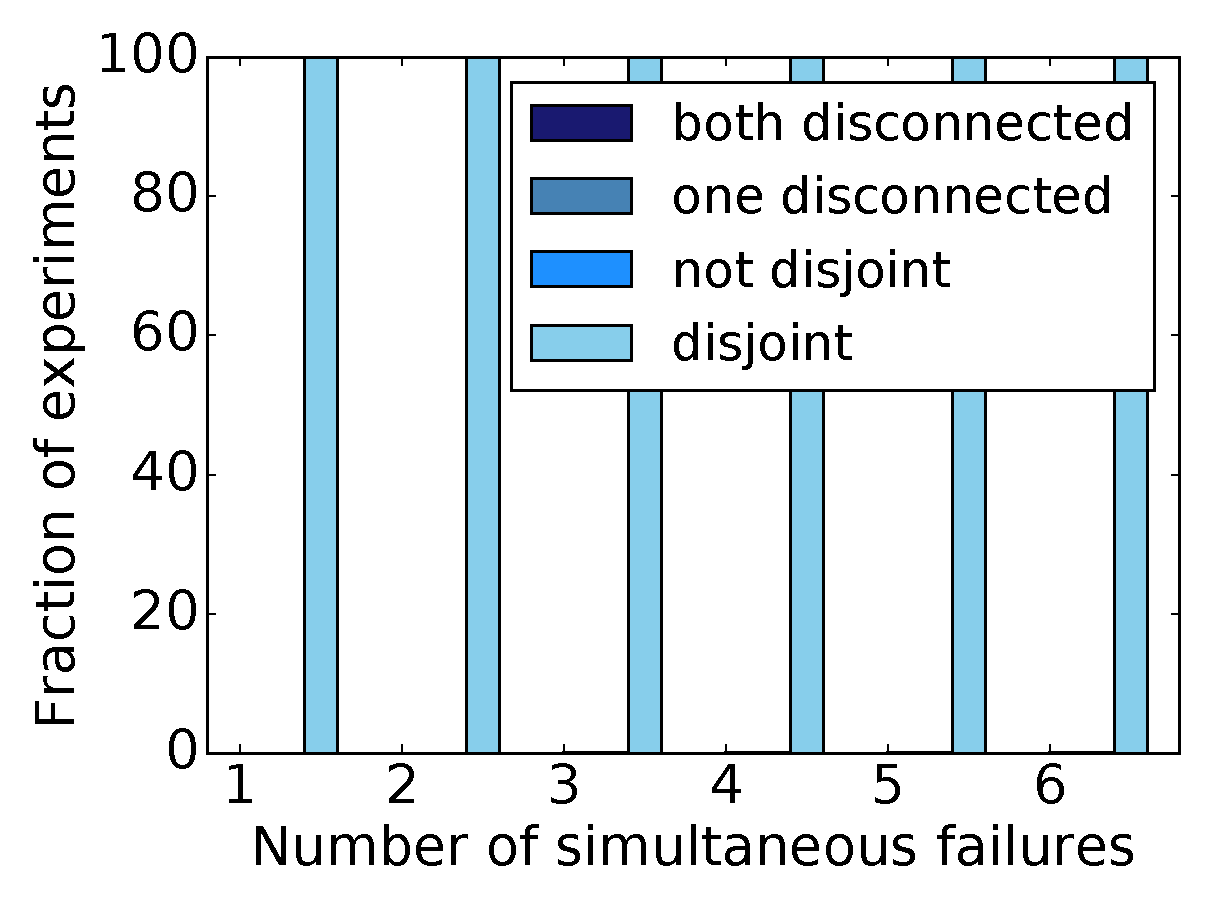
\includegraphics[width=0.45 \columnwidth]{figures/real1_random.eps}
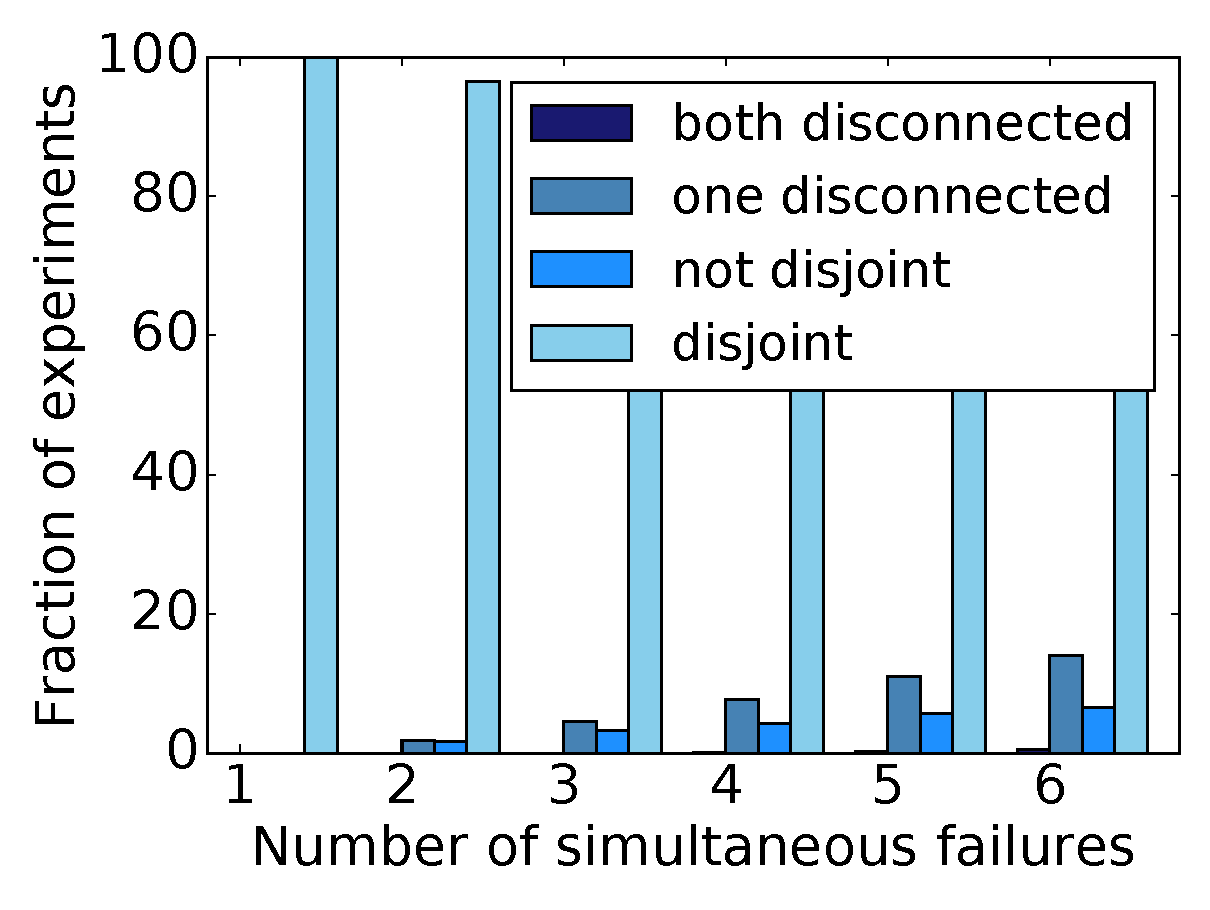
\includegraphics[width=0.45 \columnwidth]{figures/real1_worst.eps}
\end{center}
\caption{Random failures and path link failures over the worst case topoology.}
\label{fig:failure_sets_worst}
\end{figure}

\begin{figure}
\begin{center}
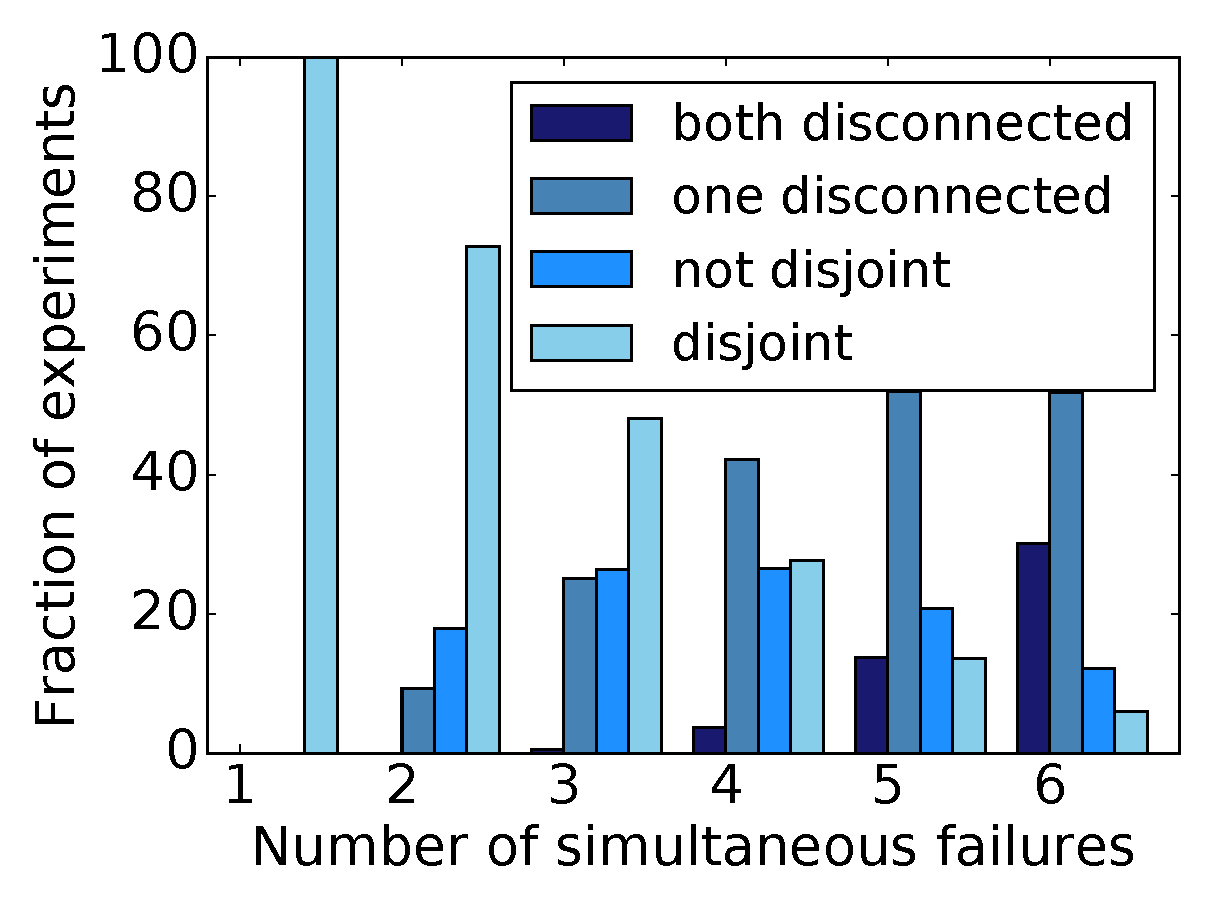
\includegraphics[width=0.45 \columnwidth]{figures/DialtelecomCz_worst.eps}
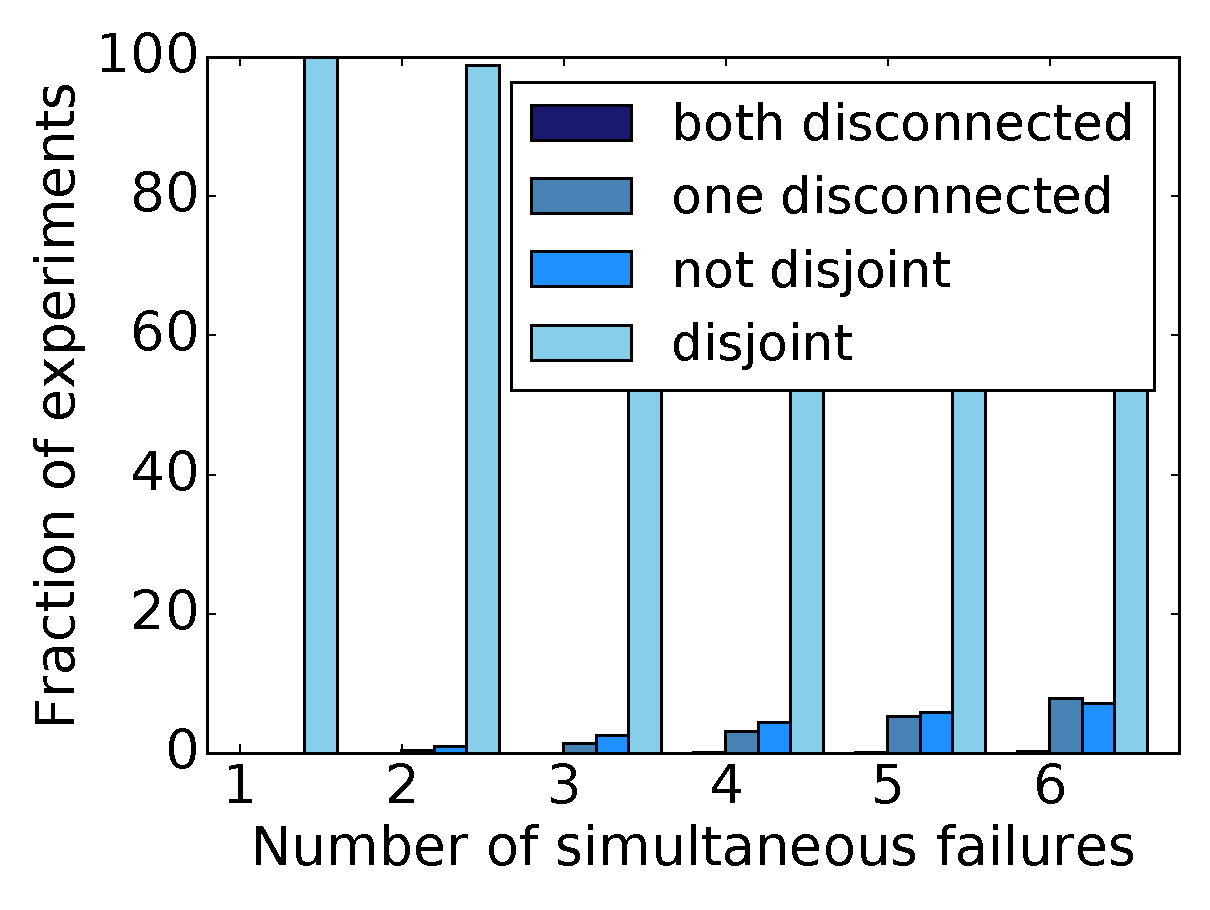
\includegraphics[width=0.45 \columnwidth]{figures/DialtelecomCz_random.eps}
\end{center}
\caption{Random failures and path link failures over the best case topology.}
\label{fig:failure_sets_best}
\end{figure}

We wondered whether we could evaluate the robustness of a pair of sr-paths algorithmically rather than 
having to perform such an experiment. The following theorem shows that it is $\NPhard$ to compute the minimum number of failures
that a pair of sr-paths can withstand until they cease to be disjoint.

\begin{problem}{Minimum cardinality failure}
\label{prob:eff-rob} 
\textbf{Input:} A network $G$ and two sr-paths $\sr{p}_1$ and $\sr{p}_2$.

\textbf{Output:} The cardinality of a minimal set of links $f \subseteq E(G)$ such that
$\sr{p}_1$ and $\sr{p}_2$ are not disjoint on $G \setminus f$.
\end{problem}

\begin{theorem}
Problem \ref{prob:eff-rob} is \NPhard. 
\end{theorem}

The following proof resulted from discussions with a student of mine, Simon Tihon, while I was coaching 
him for algorithmic programming contents.

\begin{proof}
To prove that this problem is $\NPhard$ it is enough to prove that the problem is $\NPhard$ for sr-paths of the form
$\sr{p}_1 = \langle s_1, t_1 \rangle$ and $\sr{p}_2 = \langle s_2, t_2 \rangle$. This amounts to,
given four nodes $s_1, s_2, t_1$ and $t_2$, find the minimum numbers of edges that we need to remove so that
the shortest paths from $s_1$ to $t_1$ intersect the shortest paths from $s_2$ to $t_2$.

It is known that the problem of finding the minimum number of edges that need to be removed so that the shortest path
between two given nodes becomes strictly larger than a given value $d$ is $\NPhard$ \cite{Golovach2011PathsOB}. Let $G, s, t, d$ be an instance
of this problem and assume that we can solve our problem
is polynomial time. We can assume that the shortest path between $s$ and $t$ has cost lower than or equal to $d$ or otherwise the problem is trivial.
e build an instance of Problem \ref{prob:eff-rob} by setting $s_2 = s, t_2 = t$ and adding two
nodes $s_1, t_1$. We connect $s_1$ to $s_2$ with an link of weight $d$ and $t_1$ to $t_2$ with a link of weight
$0$. Nodes $s_1$ and $t_1$ are connected with $K + 1$ parallel edges of weight $0$ where $K$ is the value of the
minimum cut between $s$ and $t$ on $G$. Figure \ref{fig:reduction} illustrates this construction.

\begin{figure}[H]
\begin{center}
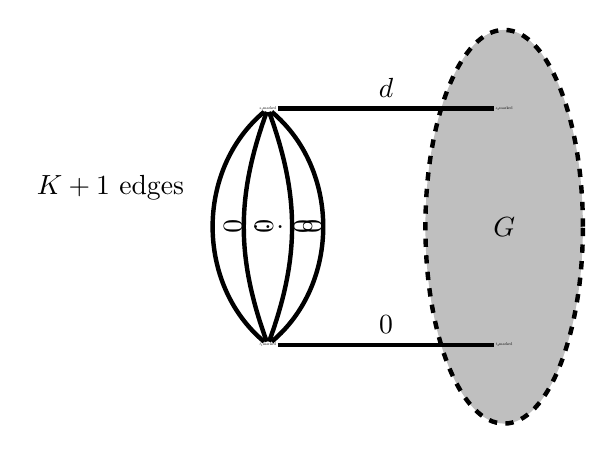
\begin{tikzpicture}
\draw[ultra thick, dashed, fill=gray!50!white] (3, -1.5) ellipse (1 and 2.5);

% \node[draw, circle, fill=lightgray] (s1) at (0, 0) {$s_1$};
% \node[draw, circle, fill=lightgray] (s2) at (3, 0) {$s_2$};
% \node[draw, circle, fill=lightgray] (t1) at (0, -3) {$t_1$};
% \node[draw, circle, fill=lightgray] (t2) at (3, -3) {$t_2$};

\node[scale=0.15] (s1) at (0,  0) {\router{$s_1$}{marked}};
\node[scale=0.15] (s2) at (3,  0) {\router{$s_2$}{marked}};
\node[scale=0.15] (t1) at (0,  -3) {\router{$t_1$}{marked}};
\node[scale=0.15] (t2) at (3,  -3) {\router{$t_2$}{marked}};


\draw (s1) edge[ultra thick, bend left = 50, sloped, above] node {$0$} (t1);
\draw (s1) edge[ultra thick, bend left = 20, sloped, above] node {$0$} (t1);
\draw (s1) edge[ultra thick, bend right = 50, sloped, above] node {$0$} (t1);
\draw (s1) edge[ultra thick, bend right = 20, sloped, above] node {$0$} (t1);

\node at (0, -1.5) {$\ldots$};

\node at (-2, -1) {$K + 1$ edges};


\draw (s1) edge[ultra thick, above] node {$d$} (s2);
\draw (t1) edge[ultra thick, above] node {$0$} (t2);


\node at (3, -1.5) {$G$};

\end{tikzpicture}
\end{center}
\caption{Construction used in the problem reduction.}
\label{fig:reduction}
\end{figure}

The shortest paths between $s_1$ and $t_1$ consists of the parallel links between them
whereas the shortest paths between $s_2 = s$ and $t_2 = t$ lie on $G$ since we assumed that the shortest
path from $s$ to $t$ has a cost lower than $d$. Note that the path visiting nodes $(s_2, s_1, t_1, t_2)$ has cost
$d$. Therefore, the shortest path from $s_2$ to $t_2$ will intersect the shortest paths from $s_1$ to $t_1$ if and only
if the shortest path from $s_1$ to $t_1$ on $G$ costs more than $d$.
Clearly, the minimum number of edges that we need to remove
so that the cost of the shortest path from $s$ to $t$ becomes at least $d$ is at most $K$ since $K$
is the value of a minimum cut (and thus a solution). Thus after removing this set the path are still well defined
since we have $K + 1$ parallel edges.
\end{proof}

\subsubsection{Evaluating existence and quality of RDPs}

In this section we will use the word detour to refer to an intermediate 
node that is in the segment stack. More concretely, for a sr-path of the form
$\langle x_1, x_2, \ldots, x_{n - 1}, x_n \rangle$, the detours are the nodes
$x_2, \ldots, x_{n - 1}$. Clearly a sr-path with $r$ detours has segment cost
$r + 2$.

We focus on reasonably well-connected \textit{source-destination
tuples}. For each topology, we randomly select 100 tuples $(s_1, s_2, t_1, t_2)$
of two sources $s_1,s_2$ and two destinations $t_1,t_2$, such that $s_1$ and
$s_2$ have a path to $t_1$ and $t_2$ even when any edge is removed. Since we try to
compute robustly disjoint paths from $s_1$ to $t_1$ and from $s_2$ to $t_2$,
it would indeed make little sense to consider source-destination pairs that are
disconnected by a single failure -- it is obvious that a service provider cannot offer
a robust connectivity service between routers that are poorly connected.
We repeat each experiment allowing between 1 and 3 detours ($k = 3, 4, 5$). We stop
at 3.

Table \ref{tab:rdp_existence} shows the percentage of these tuples for which robustly
disjoint paths exist. Sometimes, only selecting the right IGP paths is sufficient
for a given tuple. However, since IGP costs are shared across all
paths, they rarely can be used for more than one source-destination
tuple, preventing operators to configure robustly disjoint paths for
multiple customers or between different sites of the same customer.
Adding one detour by specifying an intermediate node with SR
allows paths for different tuples to be independent from each other,
solving the above issue. It also drastically increases the percentage
of tuples with at least one pair of robustly disjoint paths to 71%-100%
across all the topologies, and to 97% or more for all topologies but
two. Allowing more detours provides only slightly more flexibility
in our experiments.

\begin{figure}
\begin{center}
\begin{tabular}{ l | c c c c }
  \toprule
  & \multicolumn{3}{c}{Number of detours} \\
  Topology & 0 det & 1 det & 2 det & 3 det \\
  \midrule
  Real ISP 1 & 83\% & 100\% & 100\% & 100\% \\
  Real ISP 2 & 89\% & 100\% & 100\% & 100\% \\
  Real ISP 3 & 73\% & 100\% & 100\% & 100\% \\
  \midrule
  AS 1221 & 82\% & 98\% & 100\% & 100\% \\
  AS 1239 & 90\% & 100\% & 100\% & 100\% \\
  AS 1755 & 52\% & 98\% & 100\% & 100\% \\
  AS 3257 & 76\% & 100\% & 100\% & 100\% \\
  AS 3967 & 71\% & 99\% & 100\% & 100\% \\
  AS 6461 & 75\% & 100\% & 100\% & 100\% \\
  \midrule
  ITZ Cogentco & 78\% & 97\% & 100\% & 100\% \\ 
  ITZ Colt & 58\% & 71\% & 73\% & 73\% \\
  ITZ Deltacom & 74\% & 99\% & 99\% & 100\% \\
  ITZ Dia & 54\% & 77\% & 79\% & 79\% \\
  ITZ GtsCe & 78\% & 98\% & 100\% & 100\% \\
  ITZ Interoute & 81\% & 99\% & 100\% & 100\% \\
  ITZ Ion & 64\% & 100\% & 100\% & 100\% \\
  ITZ Tata & 86\% & 100\% & 100\% & 100\% \\
  ITZ UsCarrier & 72\% & 83\% & 85\% & 85\% \\
  \bottomrule
\end{tabular}
\end{center}
\caption{Percentage of tuples for which RDPs exist.}
\label{tab:rdp_existence}
\end{figure}

Our algorithms are designed to find sr-paths that are both
robustly disjoint and have minimal worst-path delay. As 
table \ref{tab:rdp_lat} shows, the robustly disjoint paths computed by our
algorithms have a worst-path delay which is always better than
the worst latency across the original IGP shortest paths. We are
up to 15\% more efficient, on average. Once again, more detours
enable to decrease the latency of the computed paths across all the
topologies, but just negligibly in most cases.

\begin{figure}
\begin{center}
\begin{tabular}{ l | c c c }
  \toprule
  & \multicolumn{3}{c}{Number of detours} \\
  Topology &  1 det & 2 det & 3 det \\
  \midrule
  Real ISP 1 & 0.97 & 0.97 & 0.97 \\
  Real ISP 2 & 0.98 & 0.98 & 0.98  \\
  Real ISP 3 & 0.97 & 0.96 & 0.96  \\
  \midrule
  AS 1221 & 0.99 & 0.99 & 0.99 \\
  AS 1239 & 0.97 & 0.97 & 0.97  \\
  AS 1755 & 0.90 & 0.89 & 0.88  \\
  AS 3257 & 0.91 & 0.89 & 0.88\\
  AS 3967 & 0.97 & 0.97 & 0.97  \\
  AS 6461 & 0.97 & 0.97 & 0.97  \\
  \midrule
  ITZ Cogentco & 0.85 & 0.84 & 0.84  \\ 
  ITZ Colt & 0.88 & 0.87 & 0.86  \\
  ITZ Deltacom & 0.91 & 0.90 & 0.90  \\
  ITZ Dia & 0.96 & 0.98 & 0.98  \\
  ITZ GtsCe & 0.78 & 0.77 & 0.75 \\
  ITZ Interoute & 0.93 & 0.91 & 0.90   \\
  ITZ Ion & 0.95 & 0.94 & 0.94  \\
  ITZ Tata & 0.90 & 0.89 & 0.89  \\
  ITZ UsCarrier & 0.92 & 0.92 & 0.92   \\
  \bottomrule
\end{tabular}
\end{center}
\caption{Average ratio between the RPD latency and the nominal latency.}
\label{tab:rdp_lat}
\end{figure}

To assess the benefits of robustly disjoint paths in a real-life scenario, 
we also analyse a 1-week trace of all the link-state IGP packets
exchanged by a router in Real ISP2. Based on this trace, we identified 
that a total of 5\% of the links failed during this period. Some
links experienced flapping, confirming observations of previous
studies [28, 45]. For example, one of the links failed more than 30
times during the analysed week. We select 100 source-destination
pairs in this network, and compute the corresponding robustly
disjoint paths for F = E (all single-link failures). We then replayed
all the failures that happened during the entire week. The 
source-destination pairs always have disjoint paths in our simulation, at
any moment during the week, even when multiple edges failed
simultaneously. This experiment provides a strong indication that
the paths computed by our algorithms are robust to real failures,
for a long time, in an operational network, without the need for
any configuration adjustment.


